\documentclass[dvipdfmx]{beamer}
\usepackage{bxdpx-beamer}% dvipdfmxなので必要
\usepackage{pxjahyper}% 日本語で'しおり'したい
%\usepackage{etex}
%\usetheme{Warsaw}
\usetheme{Malmoe}
%\usetheme{AnnArbor}
%\usetheme{Hannover}
%\usetheme{Bergen}
%\usetheme{Berlin}
%\usetheme{Singapore}
%\usetheme{Montpellier}
%\usetheme{Pittsburgh}
\usepackage{graphicx}
\usepackage{latexsym,amssymb}
%\usepackage{epsbox}
%\usepackage{multirow}
\usepackage{fancybox}
\usepackage{ascmac}
\usepackage{fancyvrb}
%\usepackage{listings}
\usepackage{tabularx}
\usepackage{tikz}
\usetikzlibrary{calc,shapes}
%\usepackage{pstricks,pst-node,pst-tree}
%\usepackage{multimedia}
%\usepackage{pstricks,pst-node,pst-tree}
%\usepackage{pst-all}
%\include{prooftree}
%\lstloadlanguages{pascal}
\usepackage{mathrsfs}

\renewcommand{\kanjifamilydefault}{\gtdefault}
\renewcommand{\familydefault}{\sfdefault}

\graphicspath{{figs261030/}}

%\include{cmacros}

\newcommand{\greentext}[1]{{\color[rgb]{0,0.5,0}{#1}}}
\newcommand{\redtext}[1]{{\color[rgb]{0.8,0,0}{#1}}}
\newcommand{\bluetext}[1]{{\color[rgb]{0,0,0.8}{#1}}}

\newcommand{\tuple}[1]{\langle{#1}\rangle}

\newcommand{\First}{\mathsf{First}_1}
\newcommand{\Follow}{\mathsf{Follow}_1}

%%pdt simulation

\newcommand{\pdtline}[6]{%
  \uncover<#6->{
    \node at (${#5}*(0,-.3)+(0,.3)$) {$\vdash$};%
    \node at (${#5}*(0,-.3)+(1.5,.3)$) {\parbox{12em}{(#1,}};%
    \node at (${#5}*(0,-.3)+(4.5,.3)$) {\parbox{10em}{#2,}};%
    \node at (${#5}*(0,-.3)+(5.7,.3)$) {\parbox{10em}{#3)}};%
    \node at (${#5}*(0,-.3)+(8,.3)$) {\parbox{20em}{#4}};%
  }
}

\newcommand{\initpdtline}[6]{%
  \uncover<#6->{
    \node at (${#5}*(0,-.3)+(1.5,.3)$) {\parbox{12em}{(#1,}};%
    \node at (${#5}*(0,-.3)+(4.5,.3)$) {\parbox{10em}{#2,}};%
    \node at (${#5}*(0,-.3)+(5.7,.3)$) {\parbox{10em}{#3)}};%
    \node at (${#5}*(0,-.3)+(8,.3)$) {\parbox{20em}{#4}};%
  }
}

\newtheorem{Def}{定義}
\newtheorem{Lem}{補題}
\newtheorem{Thm}{定理}
\newtheorem{Prop}{命題}

\definecolor{lightlightgrey}{rgb}{0.95,0.95,0.95}

\newcommand{\vdom}{\underline{\gg}}
\newcommand{\svdom}{\gg}

%\newcommand{\greentext}[1]{{\color[rgb]{0,0.5,0}{#1}}}
%\newcommand{\redtext}[1]{{\color[rgb]{0.8,0,0}{#1}}}

\newcommand{\lecturedate}{2026/10/30}

\cornersize{0.25}

\setbeamertemplate{frametitle}[default][center]
\setbeamertemplate{footline}{\hfill
コンパイラ\quad\lecturedate
\hfill\insertframenumber/\inserttotalframenumber\hspace*{1zw}}
\newcounter{coffee}
\setbeamercovered{transparent=10}
\title{コンパイラ(9)}
\date{\lecturedate}
\begin{document}

\frame{\titlepage}

\section{最適化}

\subsection{静的単一代入}

\begin{frame}
  \frametitle{静的単一代入を用いた最適化}

  データフロー解析のもうひとつの手法:
  静的単一代入(Static Single Assignment:SSA)\\
  \redtext{各変数の定義がプログラム中で唯一}

  変数の値は変わらないとする。二度目の代入が発生すると変数名を変更\\
  % \quad\greentext{変数を見ればUdチェーンがすぐに判明する。}\\
  \quad\greentext{値が同じの共通部分式が判別できる=式として一致}

  変換例：例6.20、6.21\\
  定義ごとに変数に添字をつける。合流する場合は、$\phi$関数で表現

  いかにして、SSA形式を得るか？
  \begin{list}{}{}
    \item [(1)] $\phi$関数の挿入
    \item [(2)] 変数の添字の決定
  \end{list}
  SSA形式において最適化
  \begin{list}{}{}
    \item [(3)] SSAから逆変換する。($\phi$関数の消去)
  \end{list}

  近年のコンパイラでよく用いられる手法

\end{frame}

\begin{frame}
  \frametitle{例}

  \begin{center}
    \begin{tabular}{c}
      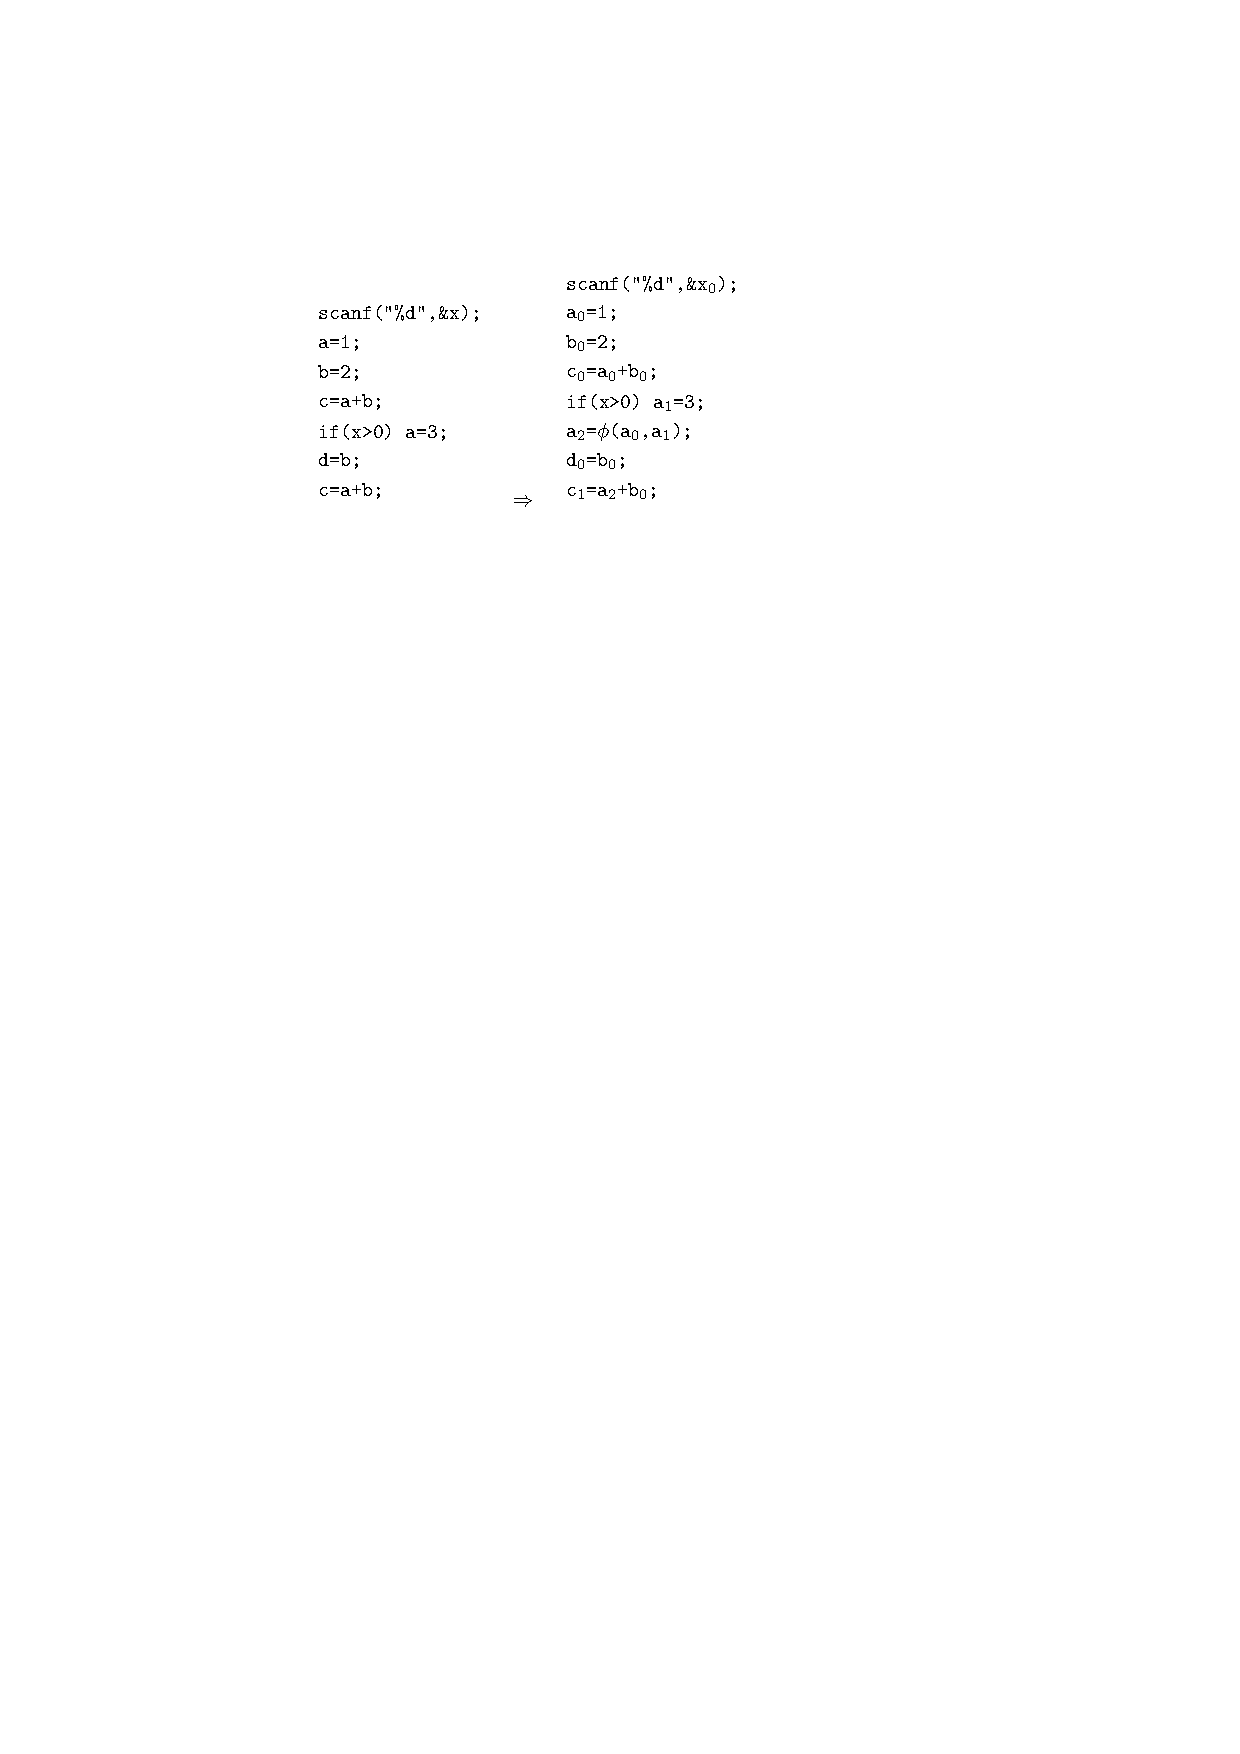
\includegraphics[height=.4\textheight]{ex6_20r1.pdf}
      \\
      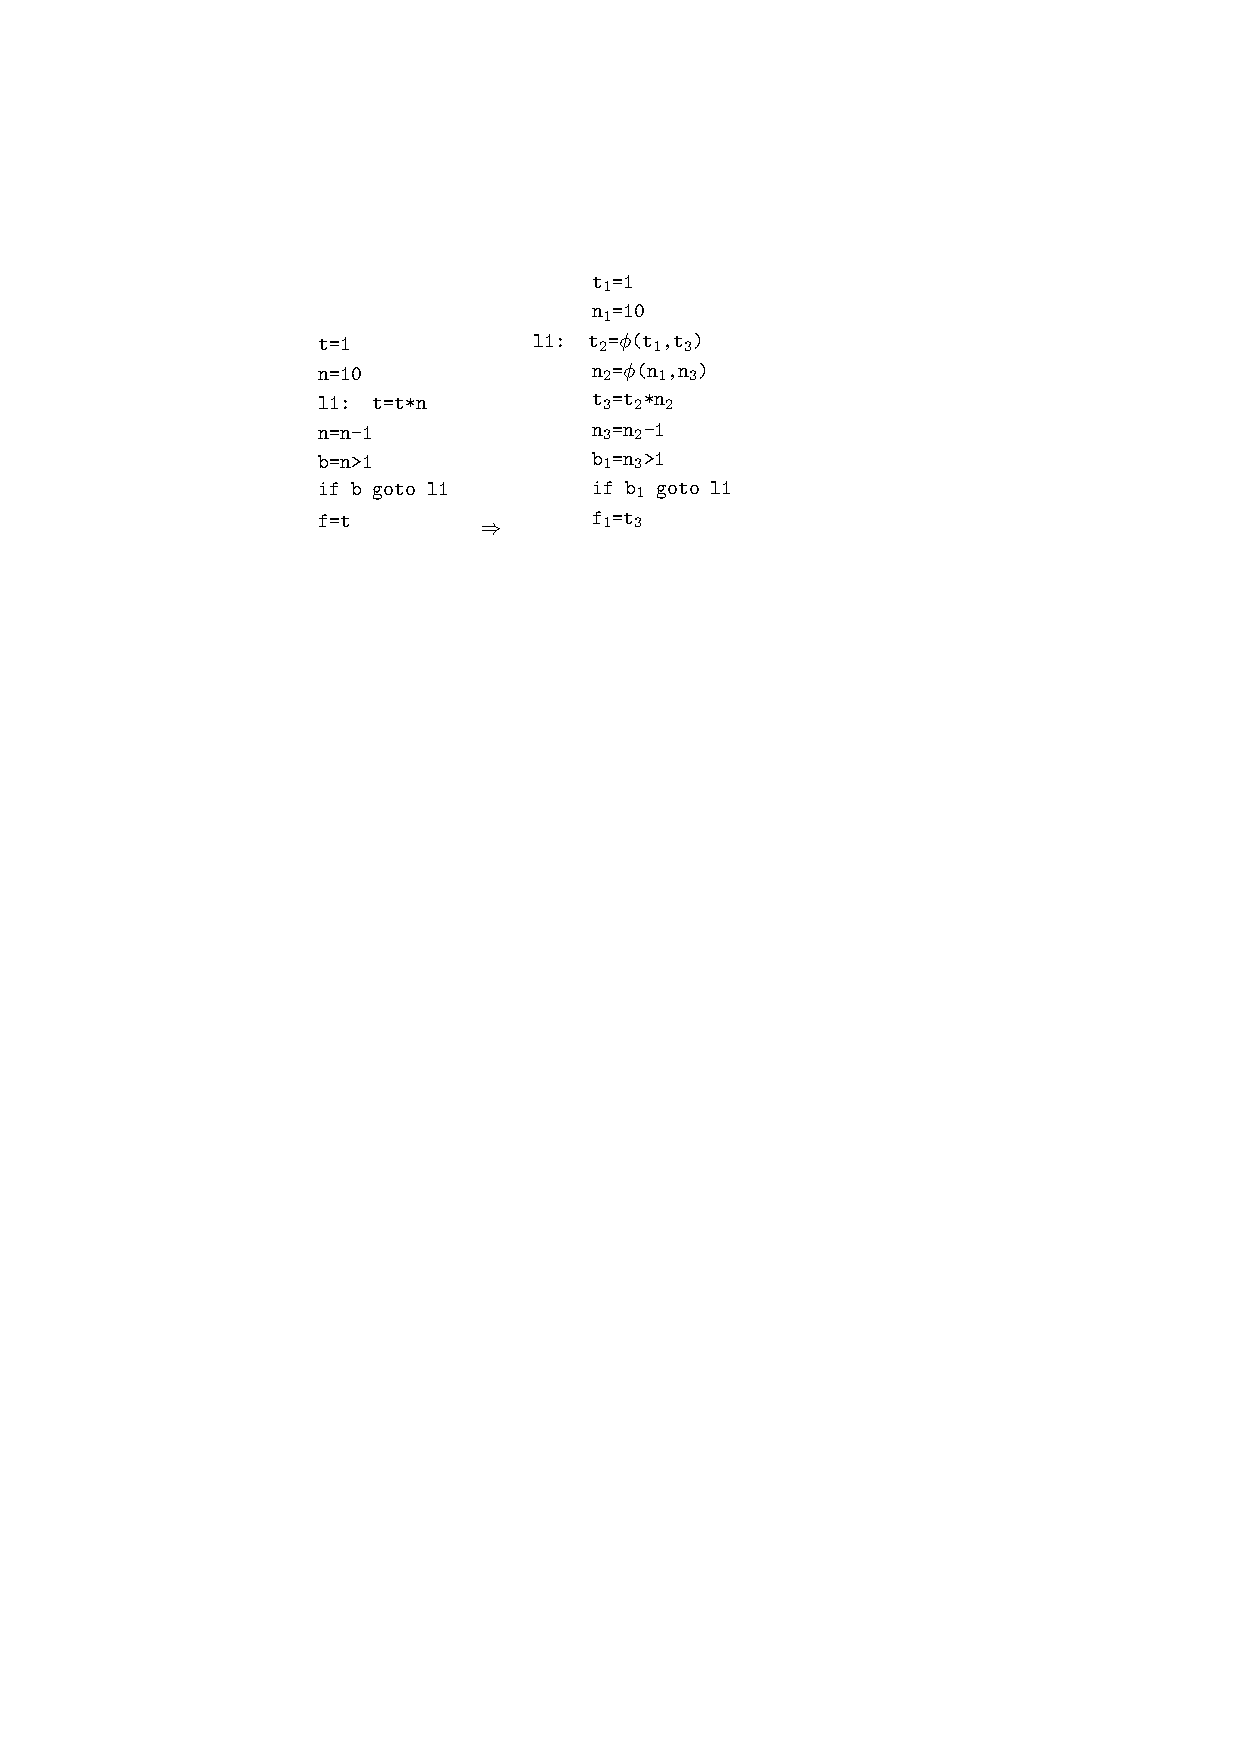
\includegraphics[height=.4\textheight]{ex6_21r1.pdf}
    \end{tabular}
  \end{center}
\end{frame}

\begin{frame}
  \frametitle{$\phi$関数の挿入}

  根つきグラフ：$(V,E)$ 先行頂点を持たない唯一の接点$v_o$(根)が存在

  \begin{center}
    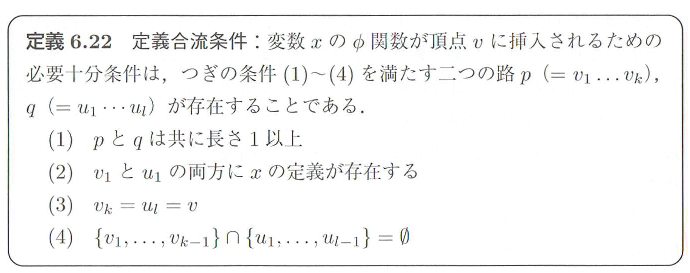
\includegraphics[width=\textwidth]{def6_22.pdf}
  \end{center}

  パス$p$上の$x$の定義=$x_1$,$q$上の$x$の定義=$x_2$
  定義合流条件の$v$に、$x_3=\phi(x_1,x_2)$
\end{frame}

\begin{frame}
  \frametitle{定義合流条件}
  \begin{center}
    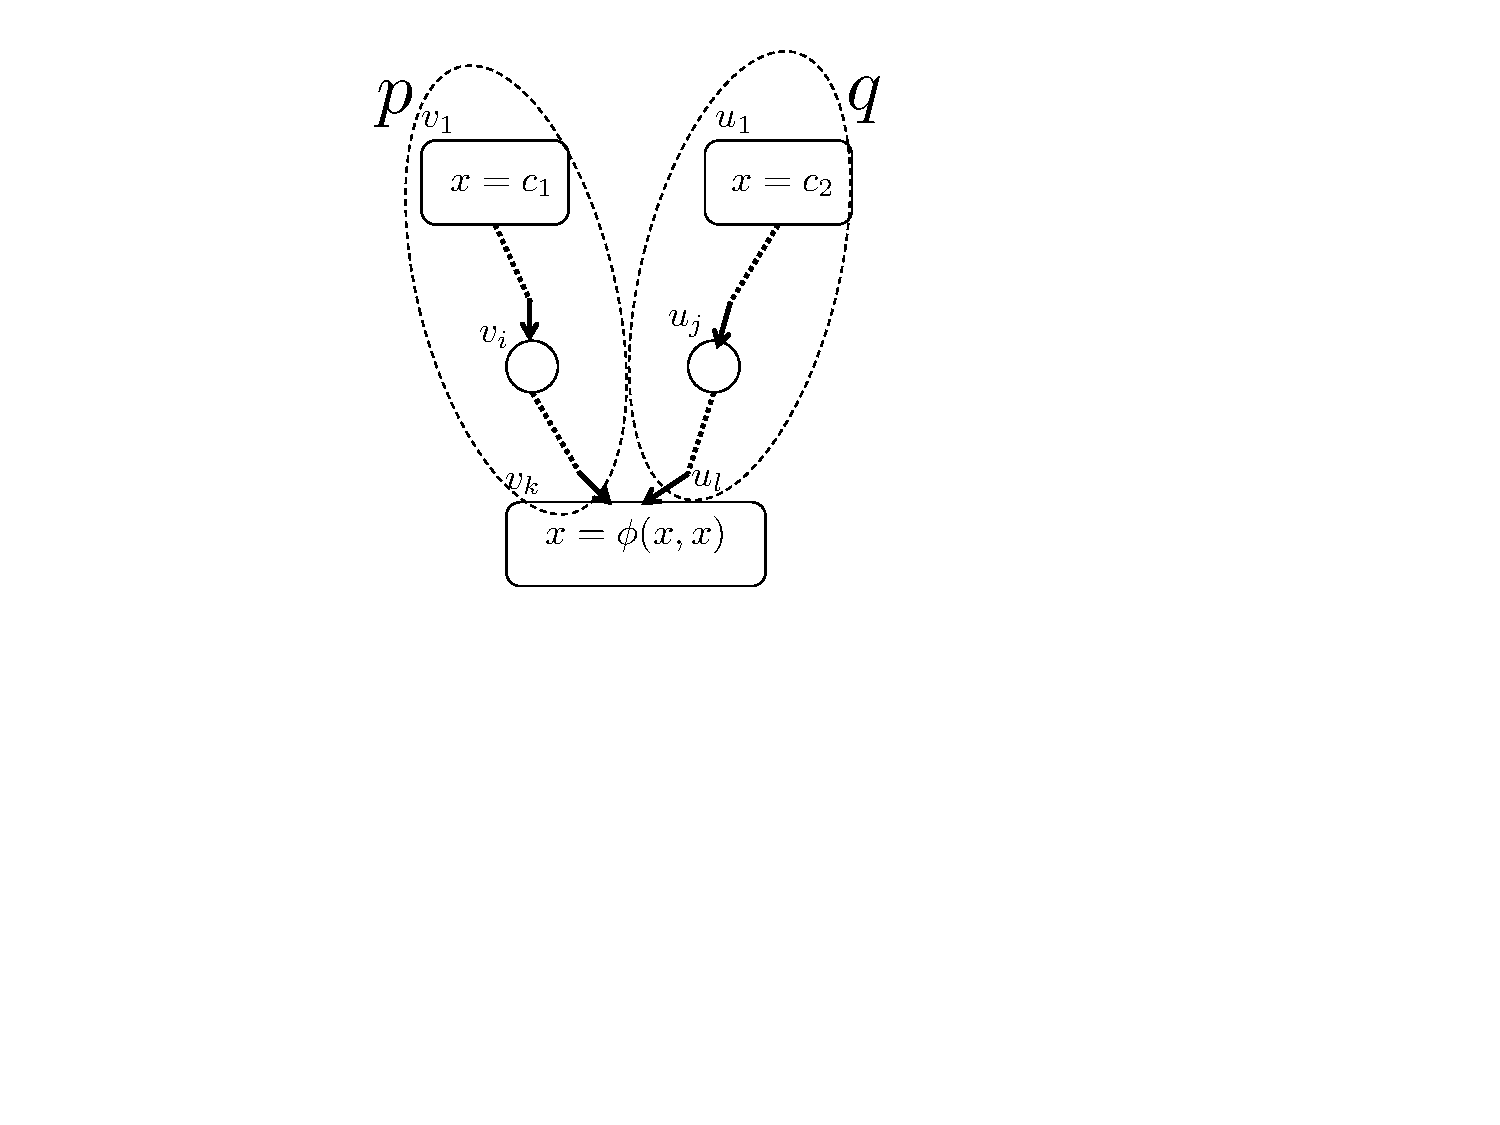
\includegraphics[width=.5\textwidth]{confluenceCondition.pdf}
  \end{center}
\end{frame}

\begin{frame}
  \frametitle{支配関係}

  支配関係：開始頂点からのパスに必ず含まれるとき、「支配」される。

  \only<1>{
    \begin{center}
      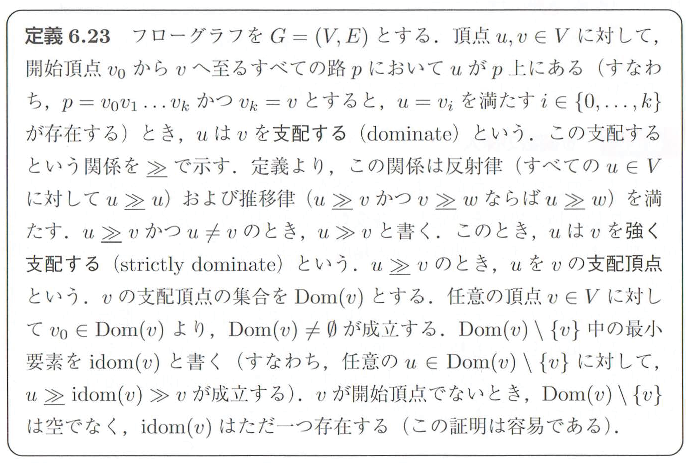
\includegraphics[width=.7\textwidth]{def6_23.pdf}
    \end{center}

    $u\underline{\gg}v$:$u$が$v$を支配:支配関係の表現=支配木 (図6.7)
  }
  \only<2>{
    \begin{center}
      \begin{tabular}{cc}

        \begin{tikzpicture}
          \node[draw,circle] (v0) at (0,3) {$v_0$};
          \node[draw,circle] (u) at (0,1.5) {$u$};
          \node[draw,circle] (v) at (0,0) {$v$};
          \node at (0,2.25) {$\cdots$};
          \node at (0,0.75) {$\cdots$};
          \path[->] (v0) [out=-30,in=30] edge (u);
          \path[->] (v0) [out=-60, in=60] edge (u);
          \path[->] (v0) [out=240,in=120] edge (u);
          \path[->] (v0) [out=210, in=150] edge (u);
          \path[->] (u) [out=-30,in=30] edge (v);
          \path[->] (u) [out=-60, in=60] edge (v);
          \path[->] (u) [out=240,in=120] edge (v);
          \path[->] (u) [out=210, in=150] edge (v);
        \end{tikzpicture}

         &
        \begin{tabular}{c}                                                         \\[-12zw]
          $u\underline{\gg}v$                                         \\[1zw]
          $u\underline{\gg}u$                                         \\
          $u\underline{\gg}v,v\underline{\gg}w$ならば$u\underline{\gg}w$ \\[1zw]
          $u\not=v$のとき$u{\gg}v$                                       \\[1zw]
          $v$以外で最も下にある支配頂点$u$: $idom(v)$                              \\[1zw]
          $(idom(v),v)$を辺とするグラフ=\redtext{支配木}
        \end{tabular}
      \end{tabular}
    \end{center}
  }
\end{frame}

\begin{frame}{フローグラフ$\rightarrow$支配木}
  \begin{tabular}{cc}
    \begin{minipage}{.4\textwidth}
      \scalebox{0.6}{
        \begin{tikzpicture}
          \node[anchor=west,draw,minimum width=3.8cm] (v0) at (0,6)
          {\small $\begin{array}{ll}\hspace*{1zw} & \mathtt{i=1}                               \\[-2pt]
                               & \mathtt{j=1}                               \\[-2pt]
                               & \mathtt{k=1}                               \\[-2pt]
                               & \mathtt{if}\ p\ \mathtt{goto}\ \mathtt{l1} \\\end{array}$};
          \node at ($(v0)+(-2.2,0.7)$) {$v_0$};
          \node[anchor=west,draw,minimum width=3.8cm] (v1) at (0,4)
          {\small $\begin{array}{ll}
                L3: & \mathtt{if}\ q\ \mathtt{goto}\ \mathtt{L2} \\
              \end{array}$};
          \node at ($(v1)+(-2.2,0)$) {$v_1$};
          \node[anchor=west,draw,minimum width=3.8cm] (v2) at (0,2.5)
          {\small $\begin{array}{ll}
                \hspace*{1zw} & \mathtt{i=i+1}   \\
                              & \mathtt{goto L3}
              \end{array}$};
          \node at ($(v2)+(-2.2,0.2)$) {$v_2$};
          \node[anchor=west,draw,minimum width=3.8cm] (v3) at (0,1)
          {\small $\begin{array}{ll}
                L1: & \mathtt{j=i+k} \\
              \end{array}$};
          \node at ($(v3)+(-2.2,0)$) {$v_3$};
          \node[anchor=west,draw,minimum width=3.8cm] (v4) at (0,0)
          {\small $\begin{array}{ll}
                L2: & \mathtt{k=i+j} \\
              \end{array}$};
          \node at ($(v4)+(-2.2,0)$) {$v_4$};
          \path[->] (v0) edge (v1);
          \path[->] (v1) edge (v2);
          \path[->] (v2) [out=210,in=150,looseness=3] edge (v1);
          \path[->] (v0) [out=350,in=10,looseness=0.5] edge (v3);
          \path[->] (v1) [out=350,in=10,looseness=0.5] edge (v4);
        \end{tikzpicture}
      }
    \end{minipage}
     &
    \begin{minipage}{.5\textwidth}
      \scalebox{0.6}{
        \begin{tikzpicture}
          \node[draw,circle] (v0) at (0,3) {$v_0$};
          \node[draw,circle] (v1) at (0,1.5) {$v_1$};
          \node[draw,circle] (v2) at (0,0) {$v_2$};
          \node[draw,circle] (v3) at (1.5,1.5) {$v_3$};
          \node[draw,circle] (v4) at (1.5,0) {$v_4$};
          \path[->] (v0) edge (v1)  (v0) edge (v3)  (v1) edge (v2)  (v1) edge (v4) (v3) edge (v4) (v2) [out=225,in=135] edge (v1);
          \node at (0.75,-1) {\small フローグラフ};

          \node[draw,circle] (w0) at (4.5,3) {$v_0$};
          \node[draw,circle] (w1) at (3,1.5) {$v_1$};
          \node[draw,circle] (w2) at (3,0) {$v_2$};
          \node[draw,circle] (w3) at (4.5,1.5) {$v_3$};
          \node[draw,circle] (w4) at (6,1.5) {$v_4$};
          \path[->] (w0) edge (w1) (w0) edge (w3) (w0) edge (w4) (w1) edge (w2);
          \node at (4.5,-1) {\small 支配木};
        \end{tikzpicture}
      }
    \end{minipage}
  \end{tabular}
\end{frame}

\begin{frame}
  \frametitle{静的単一代入を用いた最適化}

  データフロー解析のもうひとつの手法:\\
  静的単一代入(Static Single Assignment:SSA)\\
  \redtext{各変数の定義がプログラム中で唯一}

  二度目の代入が発生すると変数名を変更\\
  % \quad\greentext{変数を見ればUdチェーンがすぐに判明する。}\\
  \quad\greentext{値が同じの共通部分式が判別できる=式として一致}

  %  変換例：例6.20、6.21\\
  定義ごとに変数に添字をつける。合流する場合は、$\phi$関数で表現

  いかにして、SSA形式を得るか？

  \vspace*{5pt}

  \begin{list}{}{}
    \item [(1)] $\phi$関数の挿入
    \item [(2)] 変数の添字の決定
  \end{list}
  \par\vspace*{3pt}\par
  \qquad\redtext{SSA形式において最適化}
  \par\vspace*{3pt}\par
  \begin{list}{}{}
    \item [(3)] SSAから逆変換する。($\phi$関数の消去)
  \end{list}

  \greentext{近年のコンパイラでよく用いられる手法}

\end{frame}

\begin{frame}
  \frametitle{例}

  \begin{center}
    \begin{tabular}{c}
      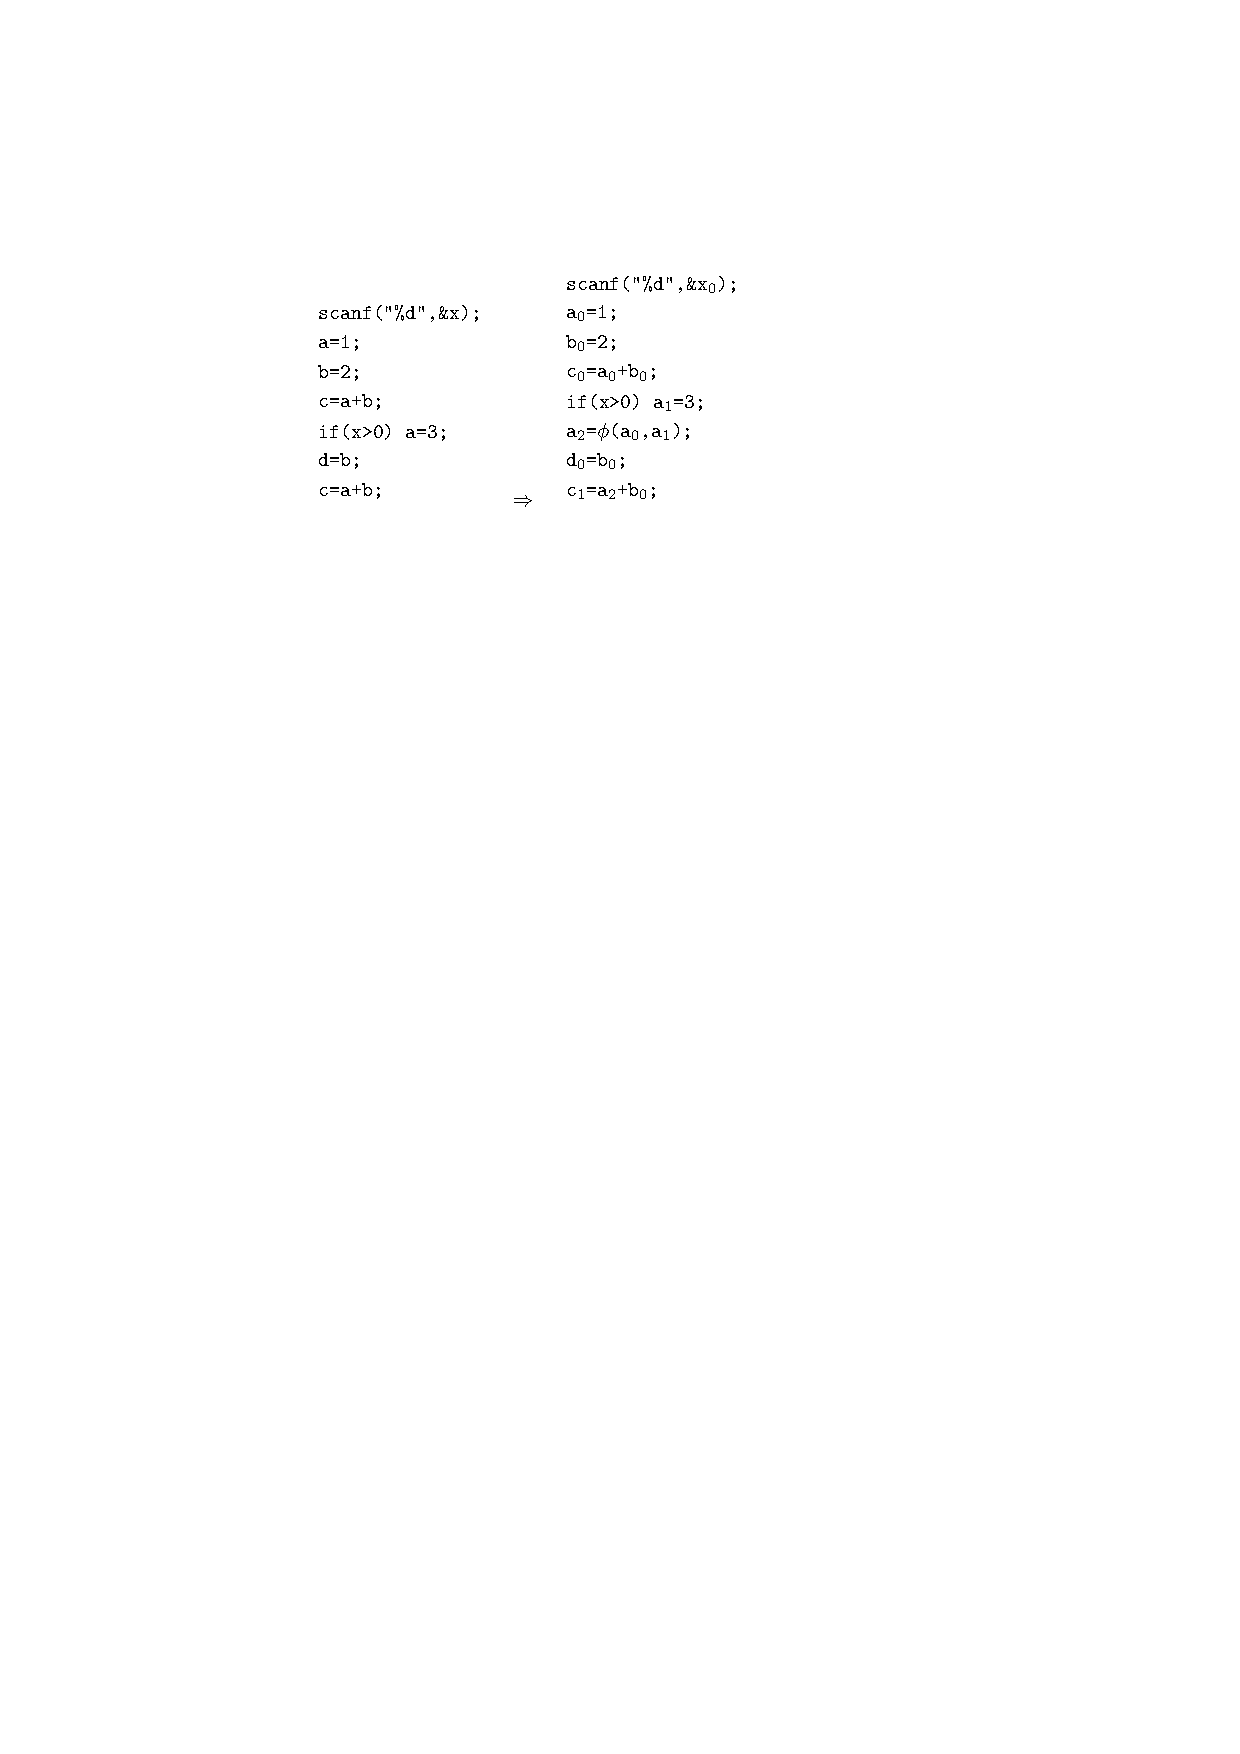
\includegraphics[height=.4\textheight]{ex6_20r1.pdf}
      \\
      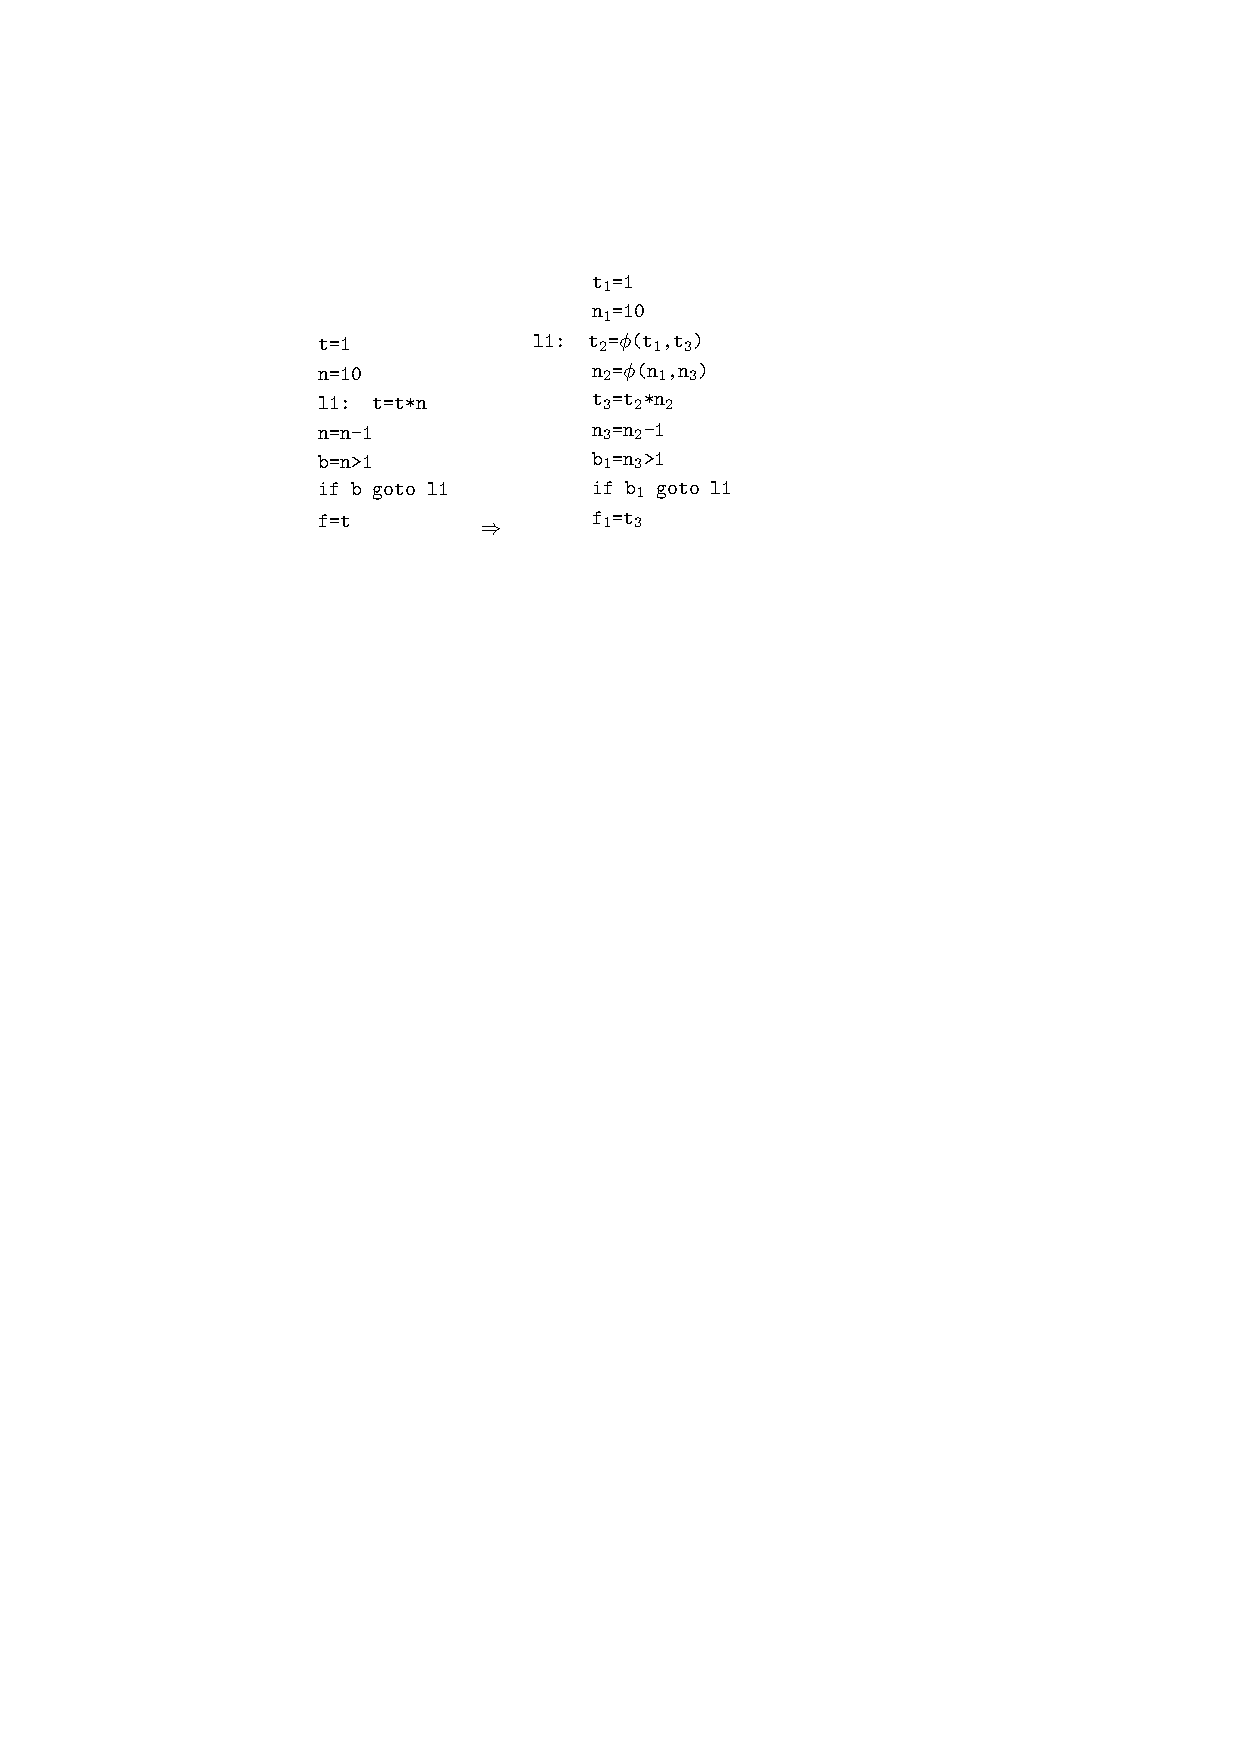
\includegraphics[height=.4\textheight]{ex6_21r1.pdf}
    \end{tabular}
  \end{center}
\end{frame}

\begin{frame}
  \frametitle{$\phi$関数の挿入}

  根つきグラフ：$(V,E)$\\
  先行頂点を持たない唯一の接点$v_o$(根)が存在

  % {\scriptsize
  \begin{itembox}[l]{定義 ({\bf 定義合流条件})}
    変数$x$の$\phi$関数が頂点$v$に挿入されるための必要十分
    条件は，次の条件(1)$\sim$(4)を満たす２つのパス$p$:$V_1,\ldots,v_k$および
    $q$:$u_1,\ldots,u_\ell$が存在することである．
    \begin{list}{(\arabic{coffee})}{\usecounter{coffee}}
      \item $k>1$, $\ell>1$
      \item $v_1$,$u_1$の両方に$x$の定義が存在
      \item $v_k=u_\ell=v$
      \item $\{v_1,\ldots,v_{k-1}\}\cap\{u_1,\ldots,u_{\ell-1}\}=\varnothing$
    \end{list}
  \end{itembox}
  % }

  %   \begin{center}
  %    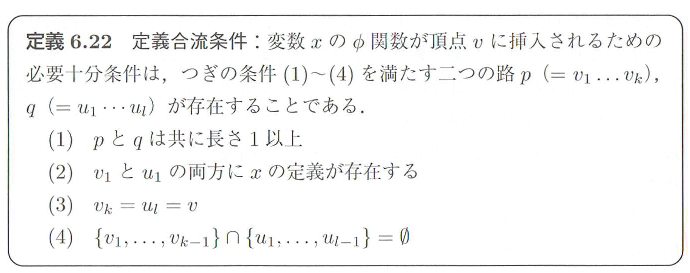
\includegraphics[width=\textwidth]{def6_22.pdf}
  %   \end{center}

  %   パス$p$上の$x$の定義=$x_1$,$q$上の$x$の定義=$x_2$
  %  定義合流条件の$v$に、$x_3=\phi(x_1,x_2)$
\end{frame}

\begin{frame}
  \frametitle{定義合流条件}
  \begin{center}
    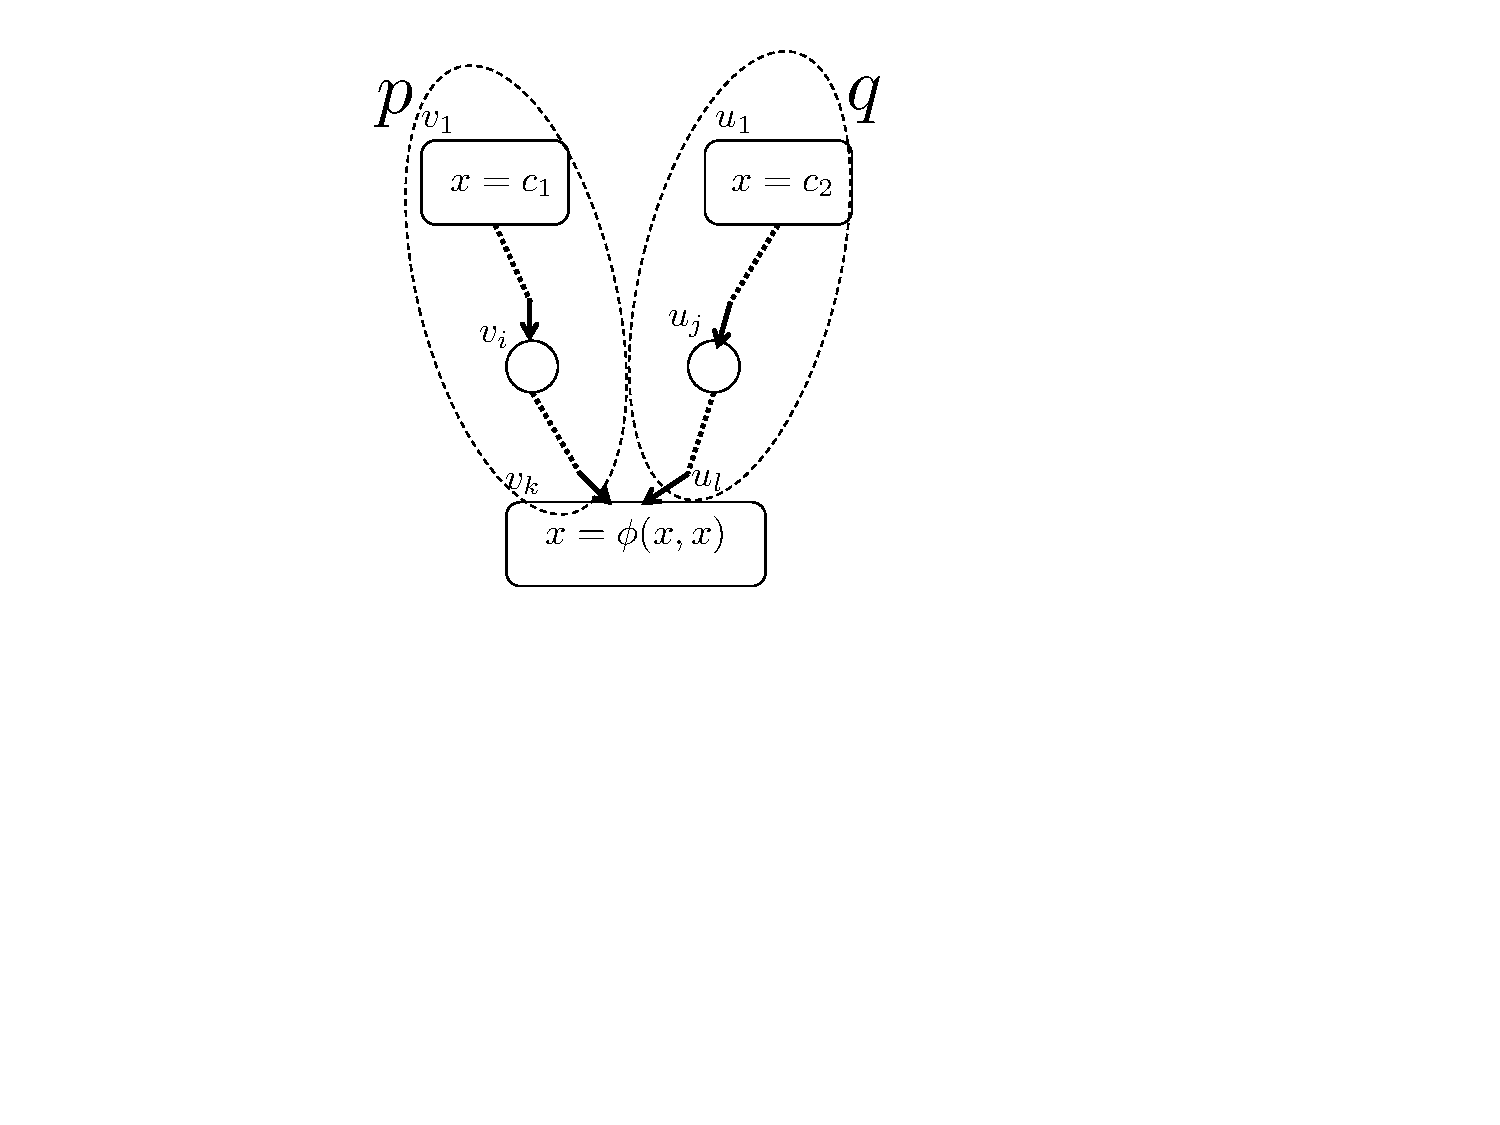
\includegraphics[width=.5\textwidth]{confluenceCondition.pdf}
  \end{center}
\end{frame}

\begin{frame}
  \frametitle{支配関係}

  {\small
    \begin{itembox}[l]{定義 (頂点間の支配関係)}
      フローグラフ$G=(V,E)$が与えられたとき，$u,v\in V$に対して，
      開始頂点$v_0$から$v$に至るすべてのパス$p:v_0,\ldots,v_k$(ここで
      $v=v_k$)において，$u\in\{v_0,\ldots,v_k\}$であるとき，
      $u$は$v$を支配するといい，$u\vdom v$と書く．
    \end{itembox}}

  {\small
    \begin{itembox}[l]{命題}
      $\vdom$は，反射率($u\vdom u$)および
      推移律($u\vdom v$かつ$v\vdom w$ならば$u\vdom w$)
      を満たす．
    \end{itembox}}

  {\small
    \begin{trivlist}
      \item $u\vdom v$かつ$u\not= v$のとき，$u$は$v$を強く支配するといい，$u\svdom v$
      と書く．
      \item $Dom(v)=\{u\,|\,u\vdom v\}$を$v$は支配頂点の集合を表す．
    \end{trivlist}
  }
\end{frame}


\begin{frame}
  \frametitle{支配関係}

  \begin{itemize}
    \item $Dom(v)\not=\varnothing$
    \item $Dom(v)\backslash\{v\}\not=\varnothing$のとき，
          唯一の$u\in Dom(v)\backslash\{v\}$が存在して，
          すべての$w\in Dom(v)\backslash\{v\}$に対して，$w\vdom u$である．\\
          （唯一性の証明）$u_1,u_2\in Dom(v)\backslash\{v\}$であるならば，開始頂点から$v$へすべてのパス上に$u_1,u_2$が存在する．よって，$u_1\vdom u_2$または
          $u_2\vdom u_1$である．したがって，$u_1=u_2$となる．\\
          このような$u$を$idom(v)$と書く．
  \end{itemize}

  \begin{itembox}[l]{(支配木)}
    有向グラフ$(V,E')$:$E=\{(idom(v),v)\,|\,v\in V\}$は，木構造となり，
    これを支配木とよぶ．
  \end{itembox}
  %支配関係：開始頂点からのパスに必ず含まれるとき、「支配」される。
\end{frame}
%   \only<1>{
%   \begin{center}
%    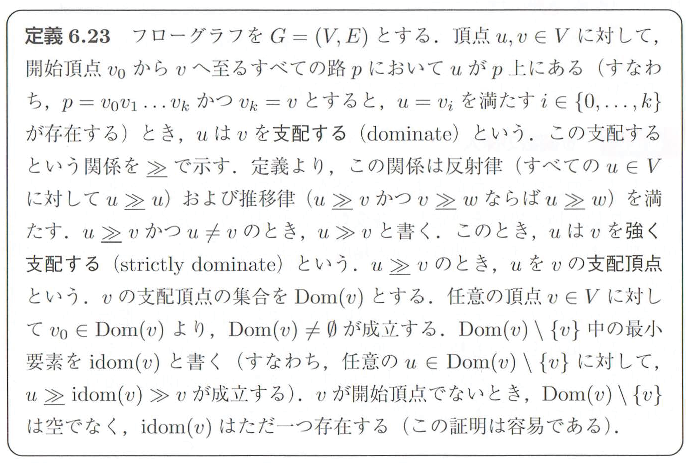
\includegraphics[width=.7\textwidth]{def6_23.pdf}
%   \end{center}

%   $u\underline{\gg}v$:$u$が$v$を支配:支配関係の表現=支配木 (図6.7)
%  }
%   \only<2>{
\begin{frame}
  \frametitle{支配関係，支配木}
  \begin{center}
    \begin{tabular}{cc}

      \begin{tikzpicture}
        \node[draw,circle] (v0) at (0,3) {$v_0$};
        \node[draw,circle] (u) at (0,1.5) {$u$};
        \node[draw,circle] (v) at (0,0) {$v$};
        \node at (0,2.25) {$\cdots$};
        \node at (0,0.75) {$\cdots$};
        \path[->] (v0) [out=-30,in=30] edge (u);
        \path[->] (v0) [out=-60, in=60] edge (u);
        \path[->] (v0) [out=240,in=120] edge (u);
        \path[->] (v0) [out=210, in=150] edge (u);
        \path[->] (u) [out=-30,in=30] edge (v);
        \path[->] (u) [out=-60, in=60] edge (v);
        \path[->] (u) [out=240,in=120] edge (v);
        \path[->] (u) [out=210, in=150] edge (v);
      \end{tikzpicture}

       &
      \begin{tabular}{c}                                                         \\[-12zw]
        $u\underline{\gg}v$                                         \\[1zw]
        $u\underline{\gg}u$                                         \\
        $u\underline{\gg}v,v\underline{\gg}w$ならば$u\underline{\gg}w$ \\[1zw]
        $u\not=v$のとき$u{\gg}v$                                       \\[1zw]
        $v$以外で最も下にある支配頂点$u$: $idom(v)$                              \\[1zw]
        $(idom(v),v)$を辺とするグラフ=\redtext{支配木}
      \end{tabular}
    \end{tabular}
  \end{center}
\end{frame}

\begin{frame}{フローグラフ$\rightarrow$支配木}
  \begin{tabular}{cc}
    \begin{minipage}{.4\textwidth}
      \scalebox{0.6}{
        \begin{tikzpicture}
          \node[anchor=west,draw,minimum width=3.8cm] (v0) at (0,6)
          {\small $\begin{array}{ll}\hspace*{1zw} & \mathtt{i=1}                               \\[-2pt]
                               & \mathtt{j=1}                               \\[-2pt]
                               & \mathtt{k=1}                               \\[-2pt]
                               & \mathtt{if}\ p\ \mathtt{goto}\ \mathtt{l1} \\\end{array}$};
          \node at ($(v0)+(-2.2,0.7)$) {$v_0$};
          \node[anchor=west,draw,minimum width=3.8cm] (v1) at (0,4)
          {\small $\begin{array}{ll}
                L3: & \mathtt{if}\ q\ \mathtt{goto}\ \mathtt{L2} \\
              \end{array}$};
          \node at ($(v1)+(-2.2,0)$) {$v_1$};
          \node[anchor=west,draw,minimum width=3.8cm] (v2) at (0,2.5)
          {\small $\begin{array}{ll}
                \hspace*{1zw} & \mathtt{i=i+1}   \\
                              & \mathtt{goto L3}
              \end{array}$};
          \node at ($(v2)+(-2.2,0.2)$) {$v_2$};
          \node[anchor=west,draw,minimum width=3.8cm] (v3) at (0,1)
          {\small $\begin{array}{ll}
                L1: & \mathtt{j=i+k} \\
              \end{array}$};
          \node at ($(v3)+(-2.2,0)$) {$v_3$};
          \node[anchor=west,draw,minimum width=3.8cm] (v4) at (0,0)
          {\small $\begin{array}{ll}
                L2: & \mathtt{k=i+j} \\
              \end{array}$};
          \node at ($(v4)+(-2.2,0)$) {$v_4$};
          \path[->] (v0) edge (v1);
          \path[->] (v1) edge (v2);
          \path[->] (v2) [out=210,in=150,looseness=3] edge (v1);
          \path[->] (v0) [out=350,in=10,looseness=0.5] edge (v3);
          \path[->] (v1) [out=350,in=10,looseness=0.5] edge (v4);
        \end{tikzpicture}
      }
    \end{minipage}
     &
    \begin{minipage}{.5\textwidth}
      \scalebox{0.6}{
        \begin{tikzpicture}
          \node[draw,circle] (v0) at (0,3) {$v_0$};
          \node[draw,circle] (v1) at (0,1.5) {$v_1$};
          \node[draw,circle] (v2) at (0,0) {$v_2$};
          \node[draw,circle] (v3) at (1.5,1.5) {$v_3$};
          \node[draw,circle] (v4) at (1.5,0) {$v_4$};
          \path[->] (v0) edge (v1)  (v0) edge (v3)  (v1) edge (v2)  (v1) edge (v4) (v3) edge (v4) (v2) [out=225,in=135] edge (v1);
          \node at (0.75,-1) {\small フローグラフ};

          \node[draw,circle] (w0) at (4.5,3) {$v_0$};
          \node[draw,circle] (w1) at (3,1.5) {$v_1$};
          \node[draw,circle] (w2) at (3,0) {$v_2$};
          \node[draw,circle] (w3) at (4.5,1.5) {$v_3$};
          \node[draw,circle] (w4) at (6,1.5) {$v_4$};
          \path[->] (w0) edge (w1) (w0) edge (w3) (w0) edge (w4) (w1) edge (w2);
          \node at (4.5,-1) {\small 支配木};
        \end{tikzpicture}
      }
    \end{minipage}
  \end{tabular}
\end{frame}

\begin{frame}
  \frametitle{支配辺境}

  フローグラフ$G=(V,E)$

  \begin{Def}
    $v$の支配辺境(Dominance Frontier)
    \[DF(v)=\{u\in V|\exists w.w\in
      pred(u),v\underline{\gg}w,v\not\gg u\}
    \]
  \end{Def}

  \greentext{強く支配していれば$\phi$関数を挿入する必要なし}

  \begin{center}
    \begin{tikzpicture}
      \draw[style=dashed] (0,0) rectangle (4,1);
      \node[draw,circle,minimum size=3mm] (u1) at (1,0.5) {};
      \node at (1,0.5) {\scriptsize $u_1$};
      \node[draw,circle,minimum size=3mm] (u2) at (2,0.5) {};
      \node at (2,0.5) {\scriptsize $u_2$};
      \node[draw,circle,minimum size=3mm] (u3) at (3,0.5) {};
      \node at (3,0.5) {\scriptsize $u_3$};

      \node[draw,circle,minimum size=3mm] (w1) at (1,2) {};
      \node at (1,2) {\scriptsize $w_1$};
      \node[draw,circle,minimum size=3mm] (w2) at (2,2) {};
      \node at (2,2) {\scriptsize $w_2$};
      \node[draw,circle,minimum size=3mm] (w3) at (3,2) {};
      \node at (3,2) {\scriptsize $w_3$};

      \node[draw,circle,minimum size=3mm] (v) at (2,3.5) {};
      \node at (2,3.5) {\scriptsize $v$};

      \node[fill,circle,minimum size=2mm] (p0) at (0,3) {};
      \node[fill,circle,minimum size=2mm] (p1) at (2.5,3.5) {};
      \node[fill,circle,minimum size=2mm] (p2) at (3.5,3) {};

      \path[->] (v) edge (w1) (v) edge (w2) (v) edge (w3)
      (w1) edge (u1) (w2) edge (u2) (w3) edge (u3)
      (p0) edge (u1) (p1) edge (u2) (p2) edge (u3);
    \end{tikzpicture}
  \end{center}

\end{frame}

\begin{frame}
  \frametitle{支配辺境の計算}

  フローグラフ$G=(V,E)$

  \begin{Lem}
    \[
      DF(v)=DF_{local}(v)\cup\bigcup_{w\in Child(v)}DF^v_{up}(w)
    \]
    ここで、

    \[
      \begin{array}{rcl}
        DF_{local}(v) & = & \{u|(v,u)\in
        E,\mathsf{idom}(u)\not=v\}                                \\
        \multicolumn{3}{p{.5\textwidth}}{
          \mbox{\greentext{$v$の次の頂点で他からのフローが存在する}}}
        \\[10pt]
        DF^v_{up}(w)  & = & \{u\in DF(w)|\mathsf{idom}(u)\not=v\} \\
        \multicolumn{3}{p{.5\textwidth}}{
        \mbox{\greentext{$w$は支配木において$v$の子で$u$から見て、}}}             \\
        \multicolumn{3}{p{.5\textwidth}}{\mbox{\greentext{
              $v$は$w$よりも上(根に近い)にある。}}}
      \end{array}
    \]

  \end{Lem}
  支配木の葉から$DF$を計算していく(p129：例)
\end{frame}

\begin{frame}
  \frametitle{定義合流条件の計算}

  \begin{list}{}{}
    \item [定義合流条件($\mathscr{S}$)]
          二つのパス $p(=v_1,\cdots,v_k)$, $q(=u_1,\cdots,u_l)$
          \begin{list}{(\arabic{coffee})}{\usecounter{coffee}}
            \item $k\ge 2$, $l\ge 2$
            \item $v_1,u_1\in S$
            \item $v_k=u_l=v$
            \item $\{v_1,\cdots,v_{k-1}\}\cap\{u_1,\cdots,u_{l-1}\}=\emptyset$
          \end{list}

          \vspace*{5pt}

    \item $J(S)=\{v|\mbox{上の条件を満たす$v$}\}$
  \end{list}

  \vspace*{5pt}

  \redtext{\small
    変数$x$が定義される場所の集合を$S$とすると
    $J(S)$は、$x$に対して最初に$\phi$関数$x=\phi(x,x)$が挿入
    される場所}

  \vspace*{5pt}

  {\small\greentext{
      $\phi$関数によって新たに定義が挿入されるため、さらに挿入が必
      要:次の漸化式で不動点$J^+(S_0)$を計算}}

  \[
    \begin{array}{rcl}
      S_{i+1}      & = & J(S_0\cup S_i)                   \\
      J^{n+1}(S_0) & = & J(S_0\cup J^n(S_0))              \\
      J^+(S_0)     & = & \lim_{n\leftarrow\infty}J^n(S_0)
    \end{array}
  \]

\end{frame}

\begin{frame}
  \frametitle{支配辺境と合流条件}

  \begin{itembox}[l]{定理}
    $DF(S)=\bigcup_{v\in S}DF(v)$のとき、
    \[
      F_{i+1}=DF(S_0\cup F_i)\quad(i\ge 0,F_0=\emptyset)
    \]
    とするとき，$DF^+(S_0)=\lim_{n\leftarrow\infty}F_n$とする．
    このとき，
    \[
      DF^+(S_0)=J^+(S_0)
    \]
  \end{itembox}

  \greentext{合流条件は支配辺境から計算可能}

\end{frame}

\begin{frame}[fragile]
  \frametitle{例6.29}

  \begin{tabular}{ccc}
    \begin{minipage}{.4\textwidth}
      \scalebox{0.8}{
        \begin{tikzpicture}
          \node[anchor=west,draw,minimum width=3.8cm] (v0) at (0,6.5)
          {\small $\begin{array}{ll}\hspace*{1zw} & \mathtt{i=1}                               \\[-2pt]
                               & \mathtt{j=1}                               \\[-2pt]
                               & \mathtt{k=1}                               \\[-2pt]
                               & \mathtt{if}\ p\ \mathtt{goto}\ \mathtt{l1} \\\end{array}$};
          \node at ($(v0)+(-2.2,0.7)$) {$v_0$};
          \only<1>{\node[anchor=west,draw,minimum width=3.8cm] (v1) at (0,4.25)
            {\small $\begin{array}{ll}
                  L3: & \mathtt{if}\ q\ \mathtt{goto}\ \mathtt{L2} \\
                \end{array}$};}
          \only<2>{
            \node[anchor=west,draw,minimum width=3.8cm] (v1) at (0,4.25)
            {\small $\begin{array}{ll}
                  L3: & \mathtt{i=}\phi\mathtt{(i,i)}              \\[-2pt]
                      & \mathtt{if}\ q\ \mathtt{goto}\ \mathtt{L2} \\
                \end{array}$};}
          \node at ($(v1)+(-2.2,0)$) {$v_1$};
          \node[anchor=west,draw,minimum width=3.8cm] (v2) at (0,2.5)
          {\small $\begin{array}{ll}
                \hspace*{1zw} & \mathtt{i=i+1}   \\
                              & \mathtt{goto L3}
              \end{array}$};
          \node at ($(v2)+(-2.2,0.2)$) {$v_2$};
          \node[anchor=west,draw,minimum width=3.8cm] (v3) at (0,1)
          {\small $\begin{array}{ll}
                L1: & \mathtt{j=i+k} \\
              \end{array}$};
          \node at ($(v3)+(-2.2,0)$) {$v_3$};
          \only<1>{
            \node[anchor=west,draw,minimum width=3.8cm] (v4) at (0,-0.5)
            {\small $\begin{array}{ll}
                  L2: & \mathtt{k=i+j} \\
                \end{array}$};}
          \only<2>{
            \node[anchor=west,draw,minimum width=3.8cm] (v4) at (0,-0.5)
            {\small $\begin{array}{ll}
                  L2: & \mathtt{i=}\phi\mathtt{(i,i)} \\
                      & \mathtt{j=}\phi\mathtt{(j,j)} \\
                      & \mathtt{k=i+j}                \\
                \end{array}$};}
          \node at ($(v4)+(-2.2,0)$) {$v_4$};
          \path[->] (v0) edge (v1);
          \path[->] (v1) edge (v2);
          \path[->] (v2) [out=210,in=150,looseness=3] edge (v1);
          \path[->] (v0) [out=350,in=10,looseness=0.5] edge (v3);
          \path[->] (v1) [out=350,in=10,looseness=0.5] edge (v4);
          \path[->] (v3) edge (v4);
        \end{tikzpicture}
      }
    \end{minipage}
     & \hspace*{1zw} &
    \begin{minipage}{.5\textwidth}
      \begin{tabular}{l}
        $i$の定義：$S_0=\{v_0,v_2\}$  \\
        $j$の定義：$S'_0=\{v_0,v_3\}$ \\
        $k$の定義：$S''_0=\{v_0,v_4\}$
      \end{tabular}

      \[
        \begin{array}{l}
          DF^+(S_0)=\{v_1,v_4\} \\
          DF^+(S'_0)=\{v_4\}    \\
          DF^+(S''_0)=\emptyset
        \end{array}
      \]
    \end{minipage}
  \end{tabular}

\end{frame}

\subsection{SSA形式への変換}

\begin{frame}
  \frametitle{SSA形式への変換}
  \begin{tabular}{cc}
    \begin{minipage}{.5\textwidth}

      \scalebox{0.8}{
        \begin{tikzpicture}
          \only<1>{\node[anchor=west,draw,minimum width=3.8cm] (v0) at (0,6.5)
            {\small $\begin{array}{ll}\hspace*{1zw}
                   & \mathtt{i=1}                               \\[-2pt]
                   & \mathtt{j=1}                               \\[-2pt]
                   & \mathtt{k=1}                               \\[-2pt]
                   & \mathtt{if}\ p\ \mathtt{goto}\ \mathtt{L1} \\\end{array}$};}
          \only<2->{\node[anchor=west,draw,minimum width=3.8cm] (v0) at (0,6.5)
            {\small $\begin{array}{ll}\hspace*{1zw}
                   & \mathtt{i_1=1}                              \\[-2pt]
                   & \mathtt{j_1=1}                              \\[-2pt]
                   & \mathtt{k_1=1}                              \\[-2pt]
                   & \mathtt{if}\ p'\ \mathtt{goto}\ \mathtt{L1} \\\end{array}$};}
          \node at ($(v0)+(-2.2,0.7)$) {$v_0$};
          \only<1>{\node[anchor=west,draw,minimum width=3.8cm] (v1) at (0,4.25)
            {\small $\begin{array}{ll}
                  L3: & \mathtt{i=}\phi\mathtt{(i,i)}              \\[-2pt]
                      & \mathtt{if}\ q\ \mathtt{goto}\ \mathtt{L2} \\
                \end{array}$};}
          \only<2>{\node[anchor=west,draw,minimum width=3.8cm] (v1) at (0,4.25)
            {\small $\begin{array}{ll}
                  L3: & \mathtt{i=}\phi\mathtt{(i_1,i)}            \\[-2pt]
                      & \mathtt{if}\ q\ \mathtt{goto}\ \mathtt{L2} \\
                \end{array}$};}
          \only<3>{\node[anchor=west,draw,minimum width=3.8cm] (v1) at (0,4.25)
            {\small $\begin{array}{ll}
                  L3: & \mathtt{i_2=}\phi\mathtt{(i_1,i)}          \\[-2pt]
                      & \mathtt{if}\ q\ \mathtt{goto}\ \mathtt{L2} \\
                \end{array}$};}
          \only<4->{\node[anchor=west,draw,minimum width=3.8cm] (v1) at (0,4.25)
            {\small $\begin{array}{ll}
                  L3: & \mathtt{i_2=}\phi\mathtt{(i_1,i_3)}        \\[-2pt]
                      & \mathtt{if}\ q\ \mathtt{goto}\ \mathtt{L2} \\
                \end{array}$};}
          \node at ($(v1)+(-2.2,0)$) {$v_1$};
          \only<1-3>{\node[anchor=west,draw,minimum width=3.8cm] (v2) at (0,2.5)
            {\small $\begin{array}{ll}
                  \hspace*{1zw} & \mathtt{i=i+1}   \\
                                & \mathtt{goto L3}
                \end{array}$};}
          \only<4->{\node[anchor=west,draw,minimum width=3.8cm] (v2) at (0,2.5)
            {\small $\begin{array}{ll}
                  \hspace*{1zw} & \mathtt{i_3=i_2+1} \\
                                & \mathtt{goto L3}
                \end{array}$};}
          \node at ($(v2)+(-2.2,0.2)$) {$v_2$};
          \only<1-4>{\node[anchor=west,draw,minimum width=3.8cm] (v3) at (0,1)
            {\small $\begin{array}{ll}
                  L1: & \mathtt{j=i+k} \\
                \end{array}$};}
          \only<5->{\node[anchor=west,draw,minimum width=3.8cm] (v3) at (0,1)
            {\small $\begin{array}{ll}
                  L1: & \mathtt{j_2=i_1+k_1} \\
                \end{array}$};}
          \node at ($(v3)+(-2.2,0)$) {$v_3$};
          \only<1,2>{\node[anchor=west,draw,minimum width=3.8cm] (v4) at (0,-0.5)
            {\small $\begin{array}{ll}
                  L2: & \mathtt{i=}\phi\mathtt{(i,i)} \\
                      & \mathtt{j=}\phi\mathtt{(j,j)} \\
                      & \mathtt{k=i+j}                \\
                \end{array}$};}
          \only<3,4,5>{\node[anchor=west,draw,minimum width=3.8cm] (v4) at (0,-0.5)
            {\small $\begin{array}{ll}
                  L2: & \mathtt{i=}\phi\mathtt{(i_2,i)} \\
                      & \mathtt{j=}\phi\mathtt{(j_1,j)} \\
                      & \mathtt{k=i+j}                  \\
                \end{array}$};}
          \only<6->{\node[anchor=west,draw,minimum width=3.8cm] (v4) at (0,-0.5)
            {\small $\begin{array}{ll}
                  L2: & \mathtt{i_4=}\phi\mathtt{(i_2,i_1)} \\
                      & \mathtt{j_3=}\phi\mathtt{(j_1,j_2)} \\
                      & \mathtt{k_2=i_4+j_3}                \\
                \end{array}$};}
          \node at ($(v4)+(-2.2,0)$) {$v_4$};
          \path[->] (v0) edge (v1);
          \path[->] (v1) edge (v2);
          \path[->] (v2) [out=210,in=150,looseness=3] edge (v1);
          \path[->] (v0) [out=350,in=10,looseness=0.5] edge (v3);
          \path[->] (v1) [out=350,in=10,looseness=0.5] edge (v4);
          \path[->] (v3) edge (v4);
        \end{tikzpicture}
      }
    \end{minipage}
     &
    \begin{minipage}{.5\textwidth}
      \begin{center}
        \begin{tikzpicture}
          \only<1-3>{\node[draw,circle,minimum size=3mm] (vt2) at (0,0) {};}
          \only<4>{\node[draw,circle,minimum size=3mm,fill=red] (vt2) at (0,0) {};}
          \only<5->{\node[draw,circle,minimum size=3mm,fill=blue] (vt2) at (0,0) {};}
          \only<1,2>{\node[draw,circle,minimum size=3mm] (vt1) at (0,1) {};}
          \only<3>{\node[draw,circle,minimum size=3mm,fill=red] (vt1) at (0,1) {};}
          \only<4->{\node[draw,circle,minimum size=3mm,fill=blue] (vt1) at (0,1) {};}
          \only<1>{\node[draw,circle,minimum size=3mm] (vt0) at (1,2) {};}
          \only<2>{\node[draw,circle,minimum size=3mm,fill=red] (vt0) at (1,2) {};}
          \only<3->{\node[draw,circle,minimum size=3mm,fill=blue] (vt0) at (1,2) {};}
          \only<1-4>{\node[draw,circle,minimum size=3mm] (vt3) at (1,1) {};}
          \only<5>{\node[draw,circle,minimum size=3mm,fill=red] (vt3) at (1,1) {};}
          \only<6->{\node[draw,circle,minimum size=3mm,fill=blue] (vt3) at (1,1) {};}
          \only<1-5>{\node[draw,circle,minimum size=3mm] (vt4) at (2,1) {};}
          \only<6->{\node[draw,circle,minimum size=3mm,fill=red] (vt4) at (2,1) {};}

          \node at (0,0) {\scriptsize $v_2$};
          \node at (0,1) {\scriptsize $v_1$};
          \node at (1,2) {\scriptsize $v_0$};
          \node at (1,1) {\scriptsize $v_3$};
          \node at (2,1) {\scriptsize $v_4$};

          \path[->] (vt0) edge (vt1) (vt0) edge (vt3) (vt0) edge (vt4) (vt1) edge (vt2);
        \end{tikzpicture}
      \end{center}
      \[
        \only<1>{\begin{array}{ll}
            stack(i)=[] & c(i)=1 \\
            stack(j)=[] & c(j)=1 \\
            stack(k)=[] & c(k)=1 \\
          \end{array}}
        \only<2>{\begin{array}{ll}
            stack(i)=[1] & c(i)=2 \\
            stack(j)=[1] & c(j)=2 \\
            stack(k)=[1] & c(k)=2 \\
          \end{array}}
        \only<3>{\begin{array}{ll}
            stack(i)=[1,2] & c(i)=3 \\
            stack(j)=[1]   & c(j)=2 \\
            stack(k)=[1]   & c(k)=2 \\
          \end{array}}
        \only<4>{\begin{array}{ll}
            stack(i)=[1,2,3] & c(i)=4 \\
            stack(j)=[1]     & c(j)=2 \\
            stack(k)=[1]     & c(k)=2 \\
          \end{array}}
        \only<5>{\begin{array}{ll}
            stack(i)=[1,2,3] & c(i)=4 \\
            stack(j)=[1,2]   & c(j)=3 \\
            stack(k)=[1]     & c(k)=2 \\
          \end{array}}
        \only<6>{\begin{array}{ll}
            stack(i)=[1,2,3] & c(i)=4 \\
            stack(j)=[1,2]   & c(j)=3 \\
            stack(k)=[1,2]   & c(k)=3 \\
          \end{array}}
      \]
    \end{minipage}
  \end{tabular}
\end{frame}

\subsection{SSA形式に対する最適化}

\begin{frame}
  \frametitle{SSA形式に対する最適化}
  SSA形式：データフロー解析ずみのプログラム\\[2zw]

  \greentext{構文的にフローが表現されている}
  $\Rightarrow$
  \redtext{最適化を効果的に適用できる}：
  \greentext{更新のチェックが不要}

  例：DAGの構成が容易

  \vspace*{1zw}

  \begin{itemize}
    \item 定数伝播
    \item コピー伝播
    \item 共通部分式の削除
    \item ループ不変コードの移動
    \item 不用コードの削除
  \end{itemize}
\end{frame}

\begin{frame}
  \frametitle{SSA最適化例 [佐々:06]}

  \only<1>{
    \begin{center}
      \begin{tabular}{ccc}
        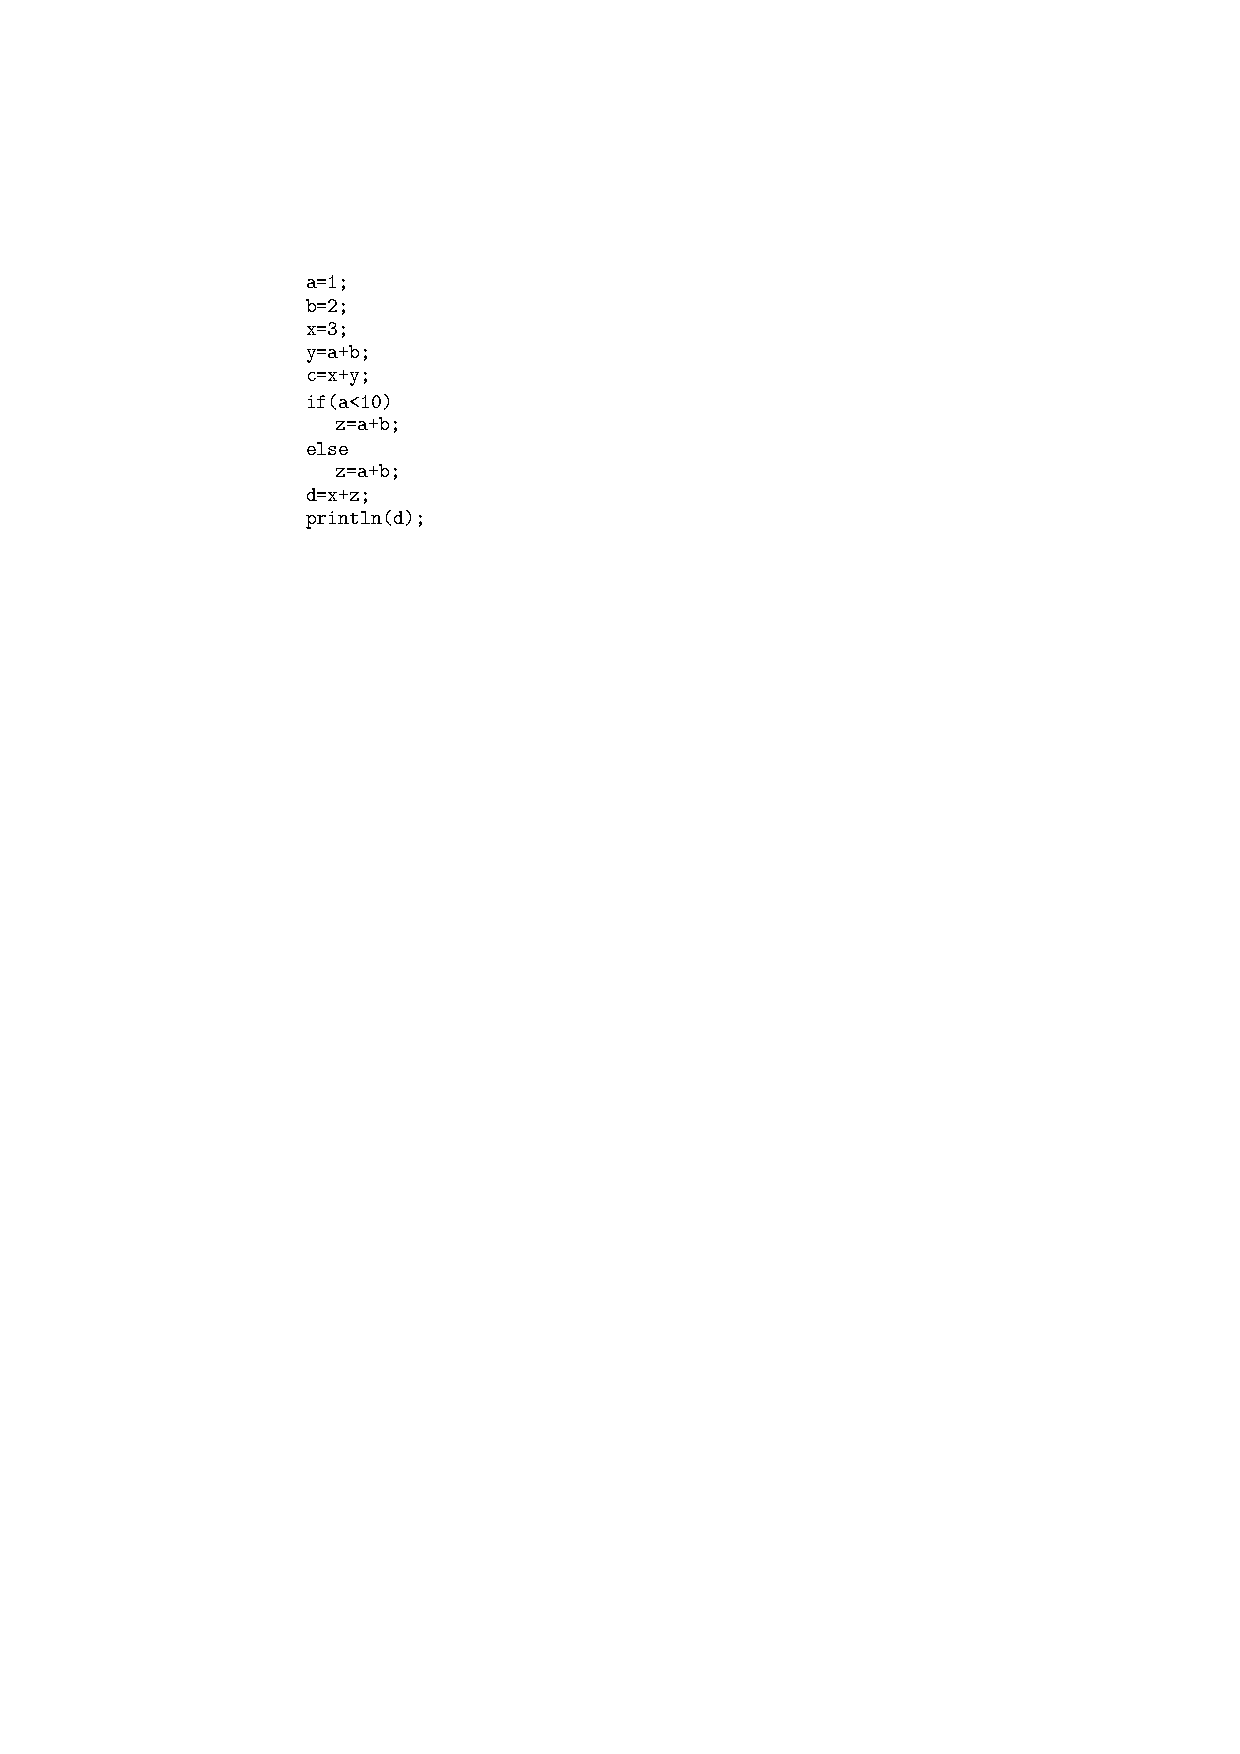
\includegraphics{ssasrc01.pdf}
         & $\Rightarrow$ &
        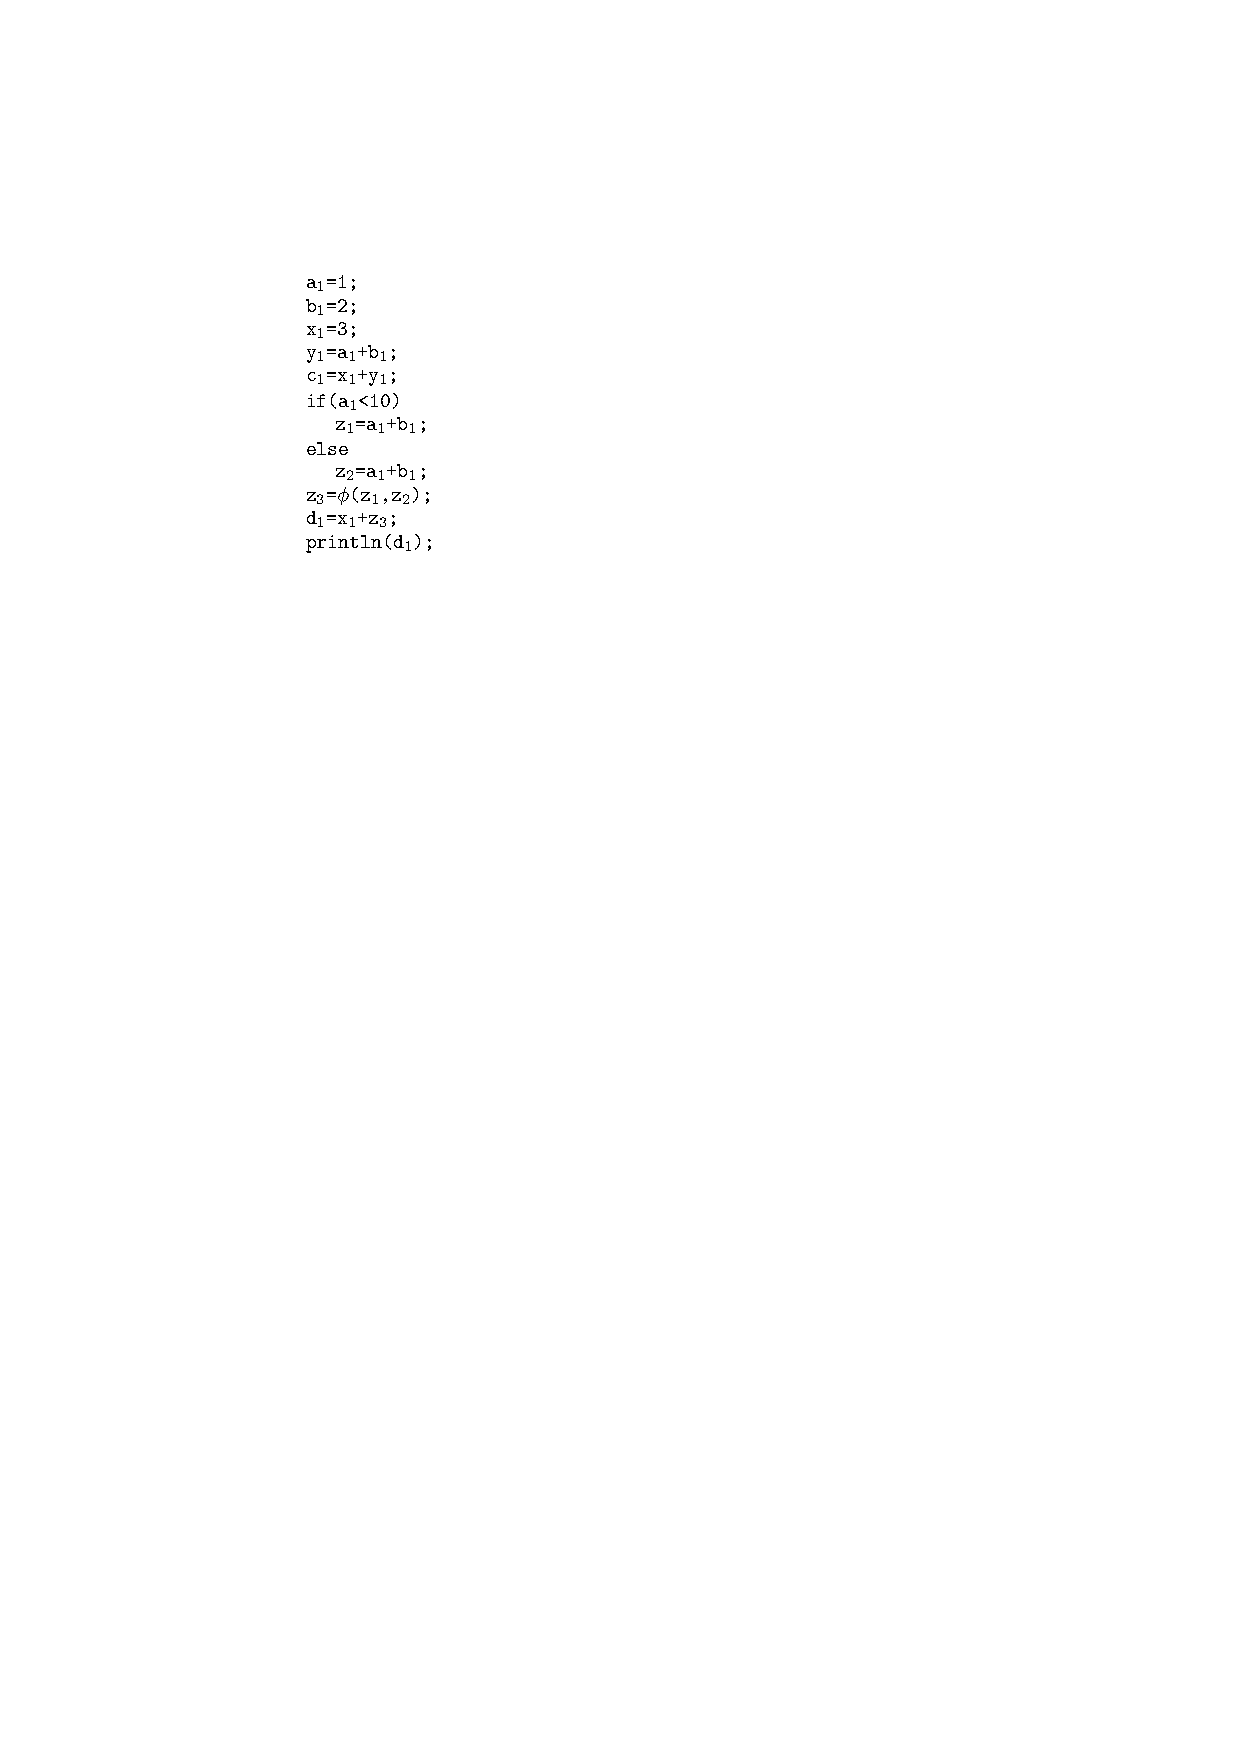
\includegraphics{ssasrc02.pdf}
        \\[1zw]
        \multicolumn{3}{c}{\greentext{SSA形式へ変換}}
      \end{tabular}
    \end{center}
  }

  \only<2>{
    \begin{center}
      \begin{tabular}{ccc}
        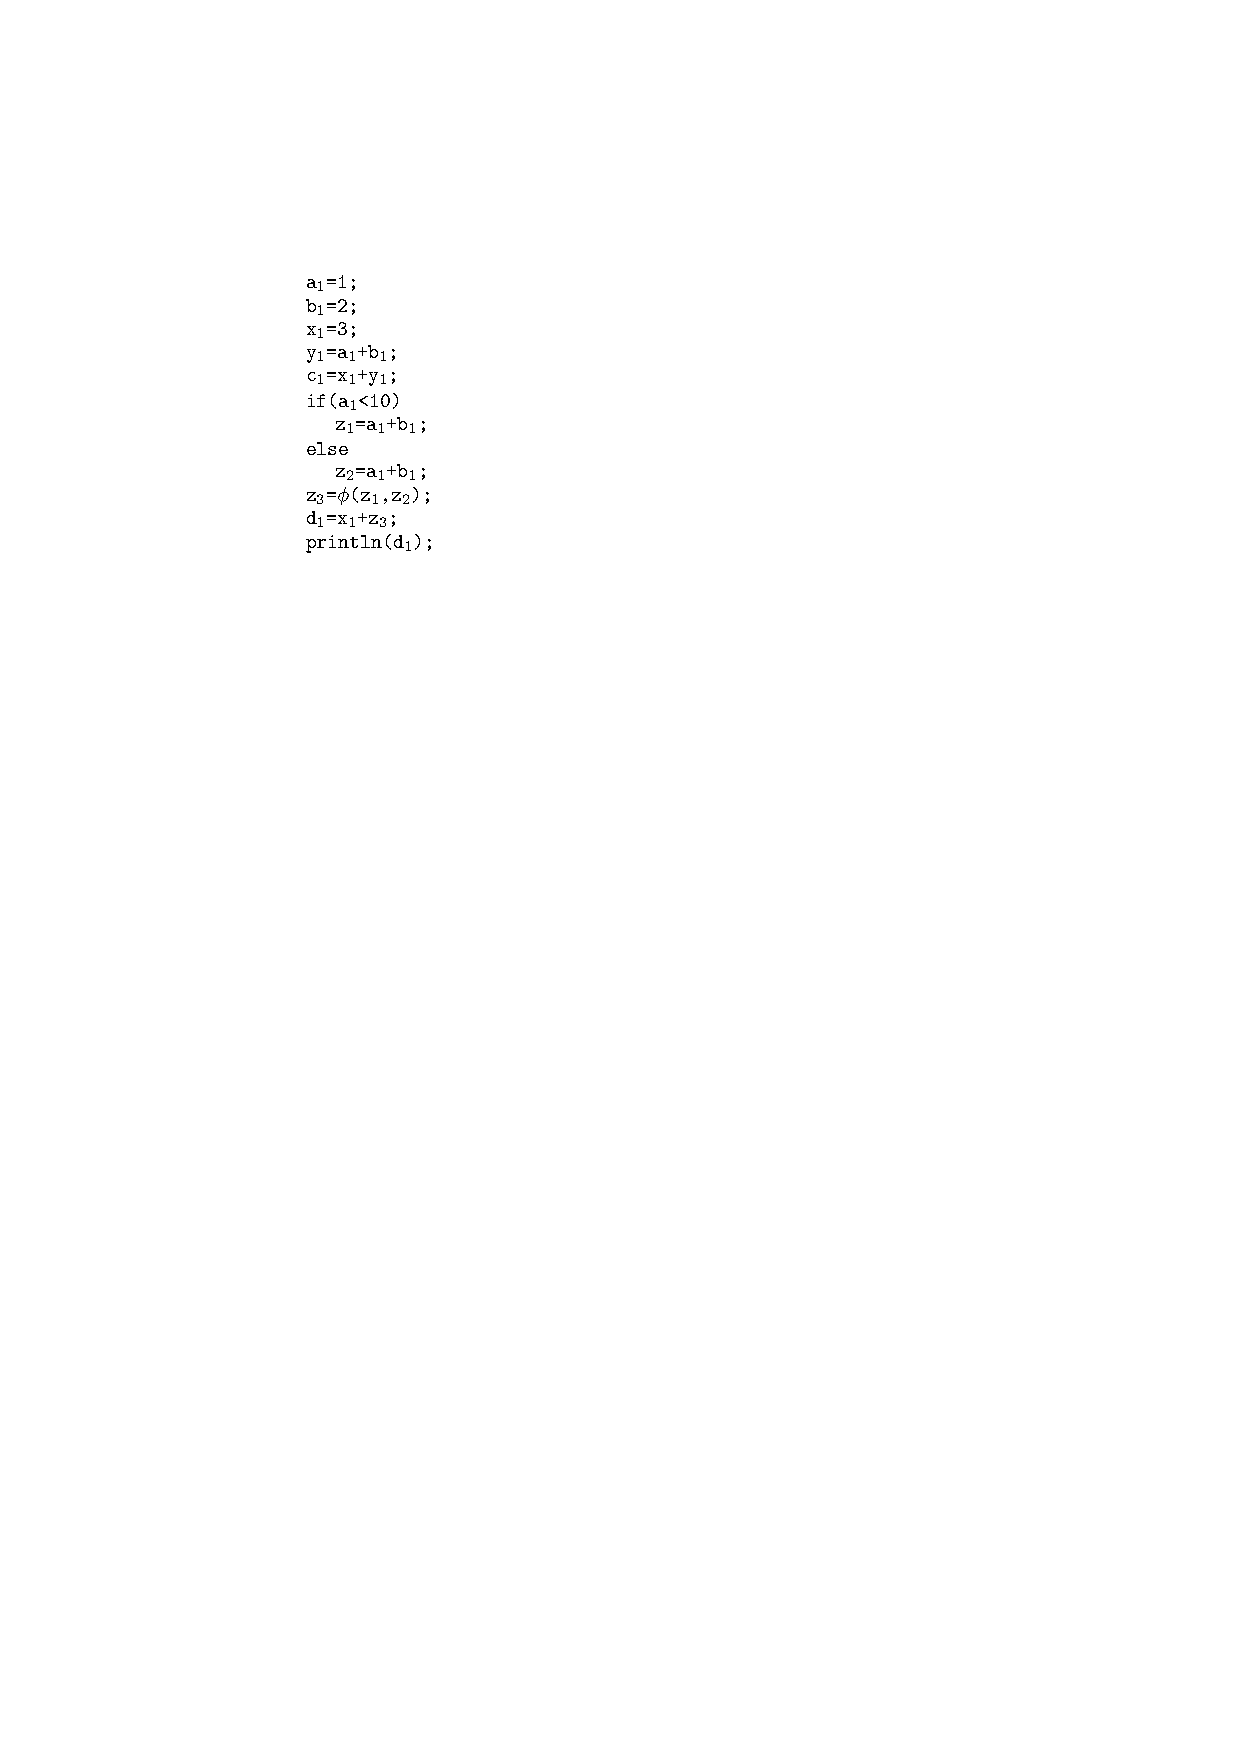
\includegraphics{ssasrc02.pdf}
         & \hspace*{1zw}$\Rightarrow$\hspace*{1zw} &
        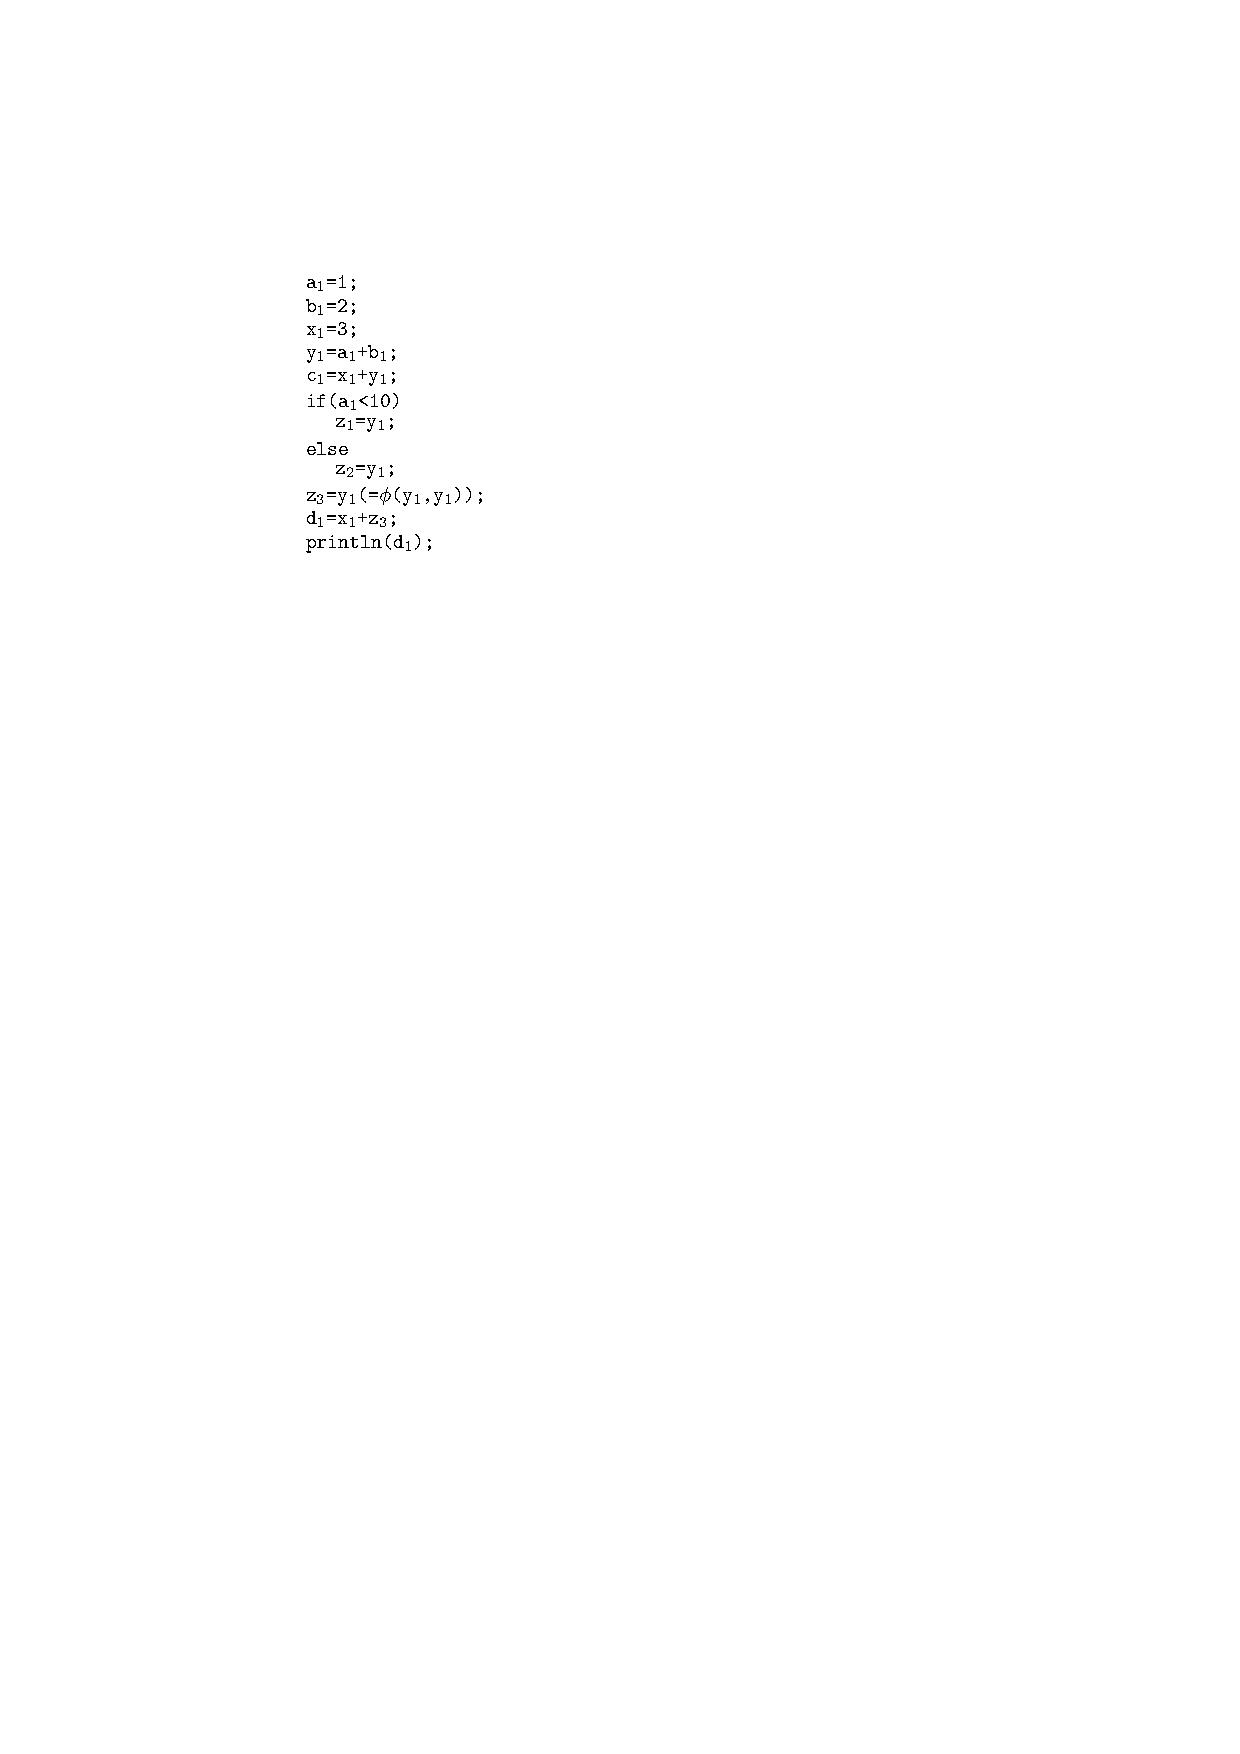
\includegraphics{ssasrc03.pdf}               \\[1zw]
        \multicolumn{3}{c}{\greentext{共通部分式除去}}
      \end{tabular}
    \end{center}
  }

  \only<3>{
    \begin{center}
      \begin{tabular}{ccc}
        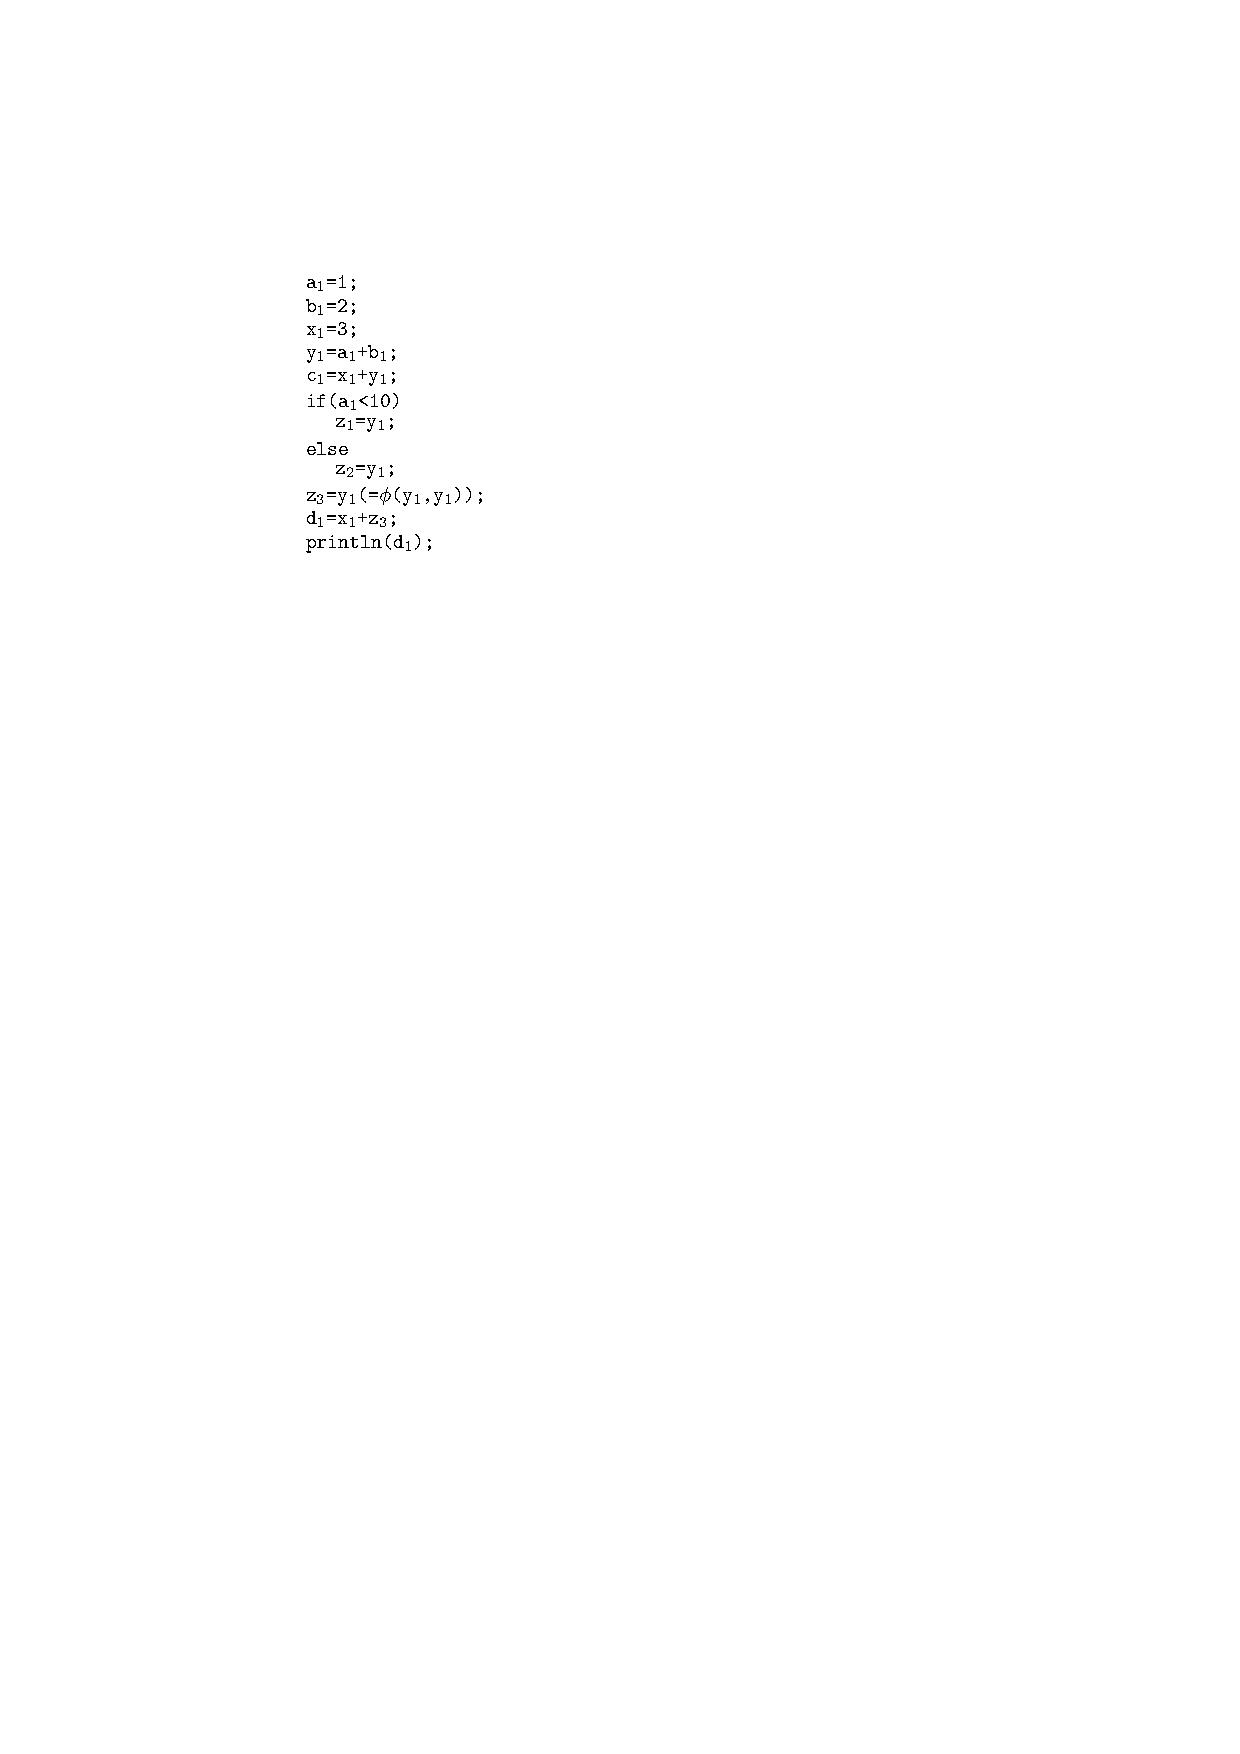
\includegraphics{ssasrc03.pdf}
         & \hspace*{1zw}$\Rightarrow$\hspace*{1zw} &
        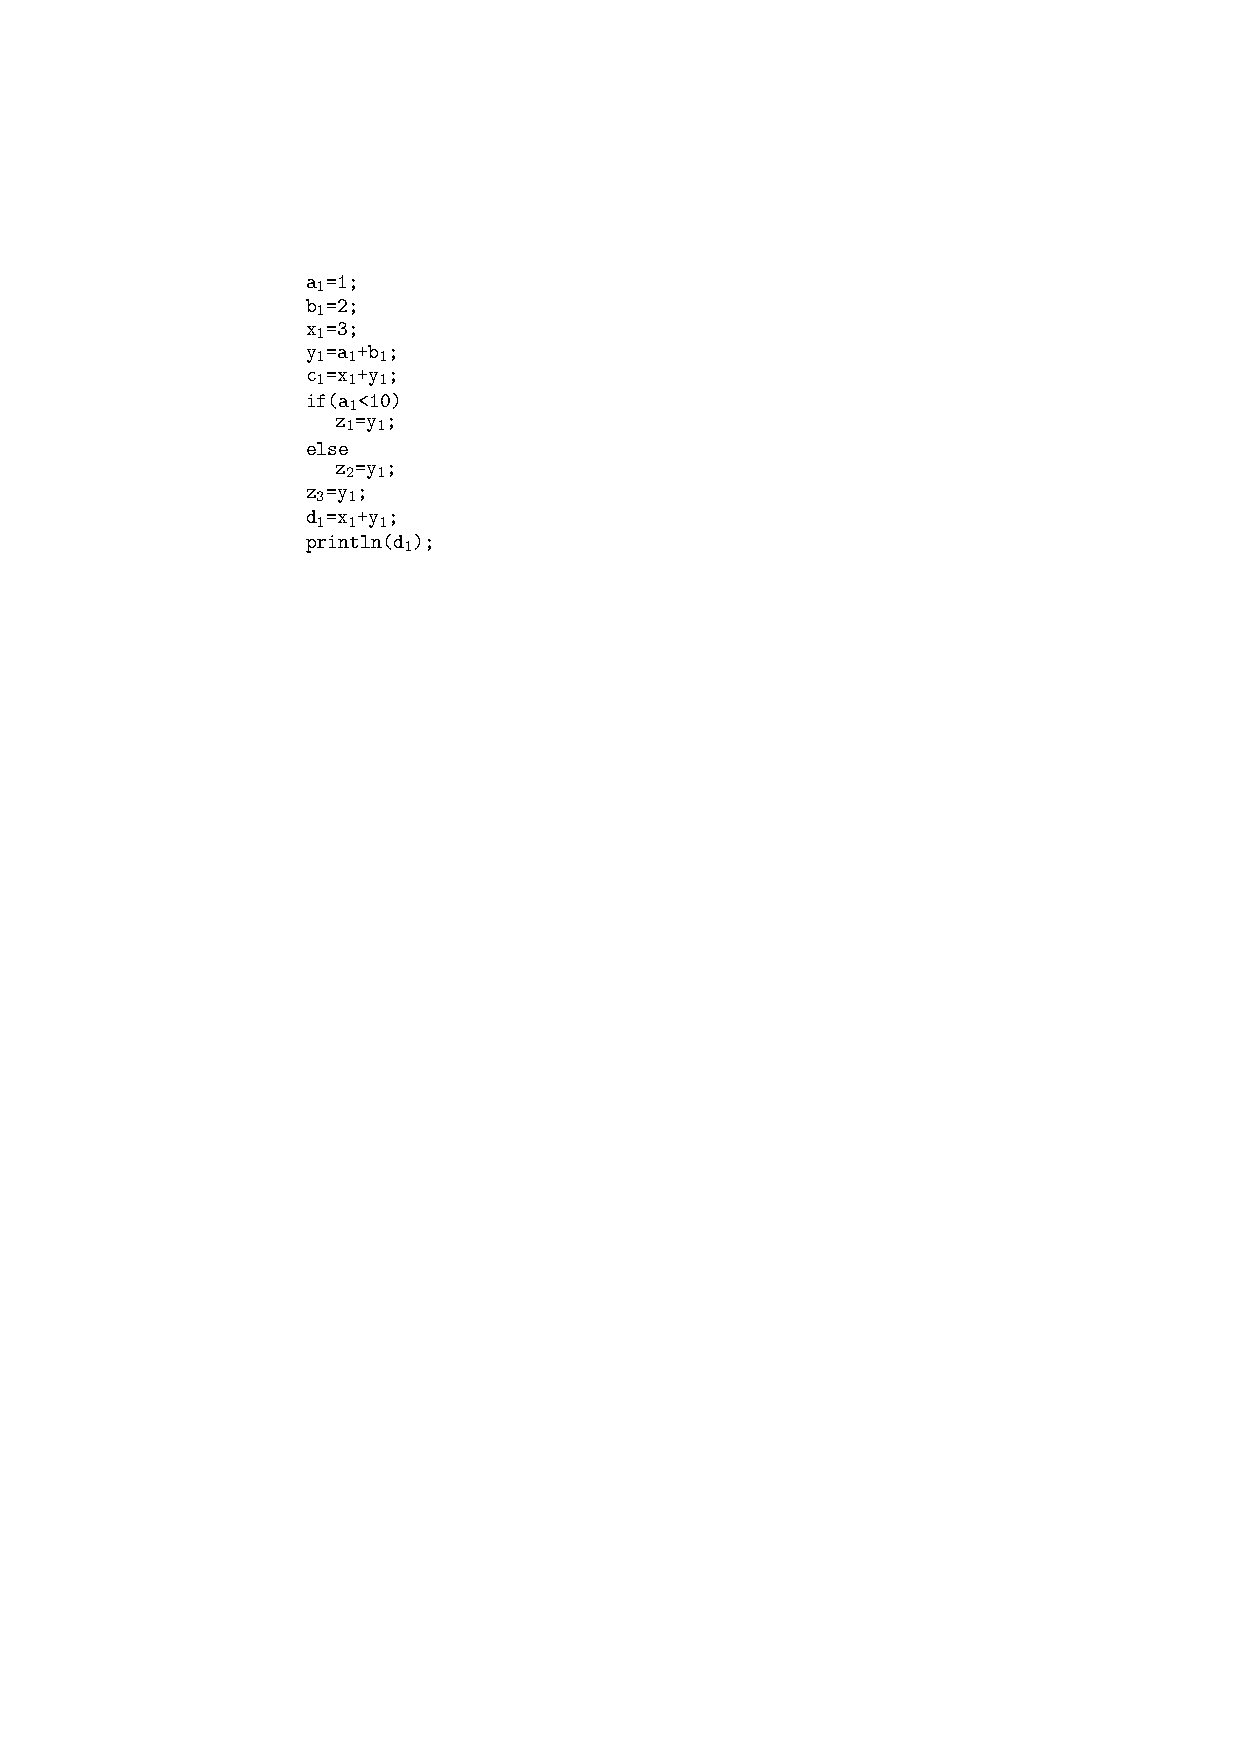
\includegraphics{ssasrc04.pdf}               \\[1zw]
        \multicolumn{3}{c}{\greentext{コピー伝播}}
      \end{tabular}
    \end{center}
  }

  \only<4>{
    \begin{center}
      \begin{center}
        \begin{tabular}{ccc}
          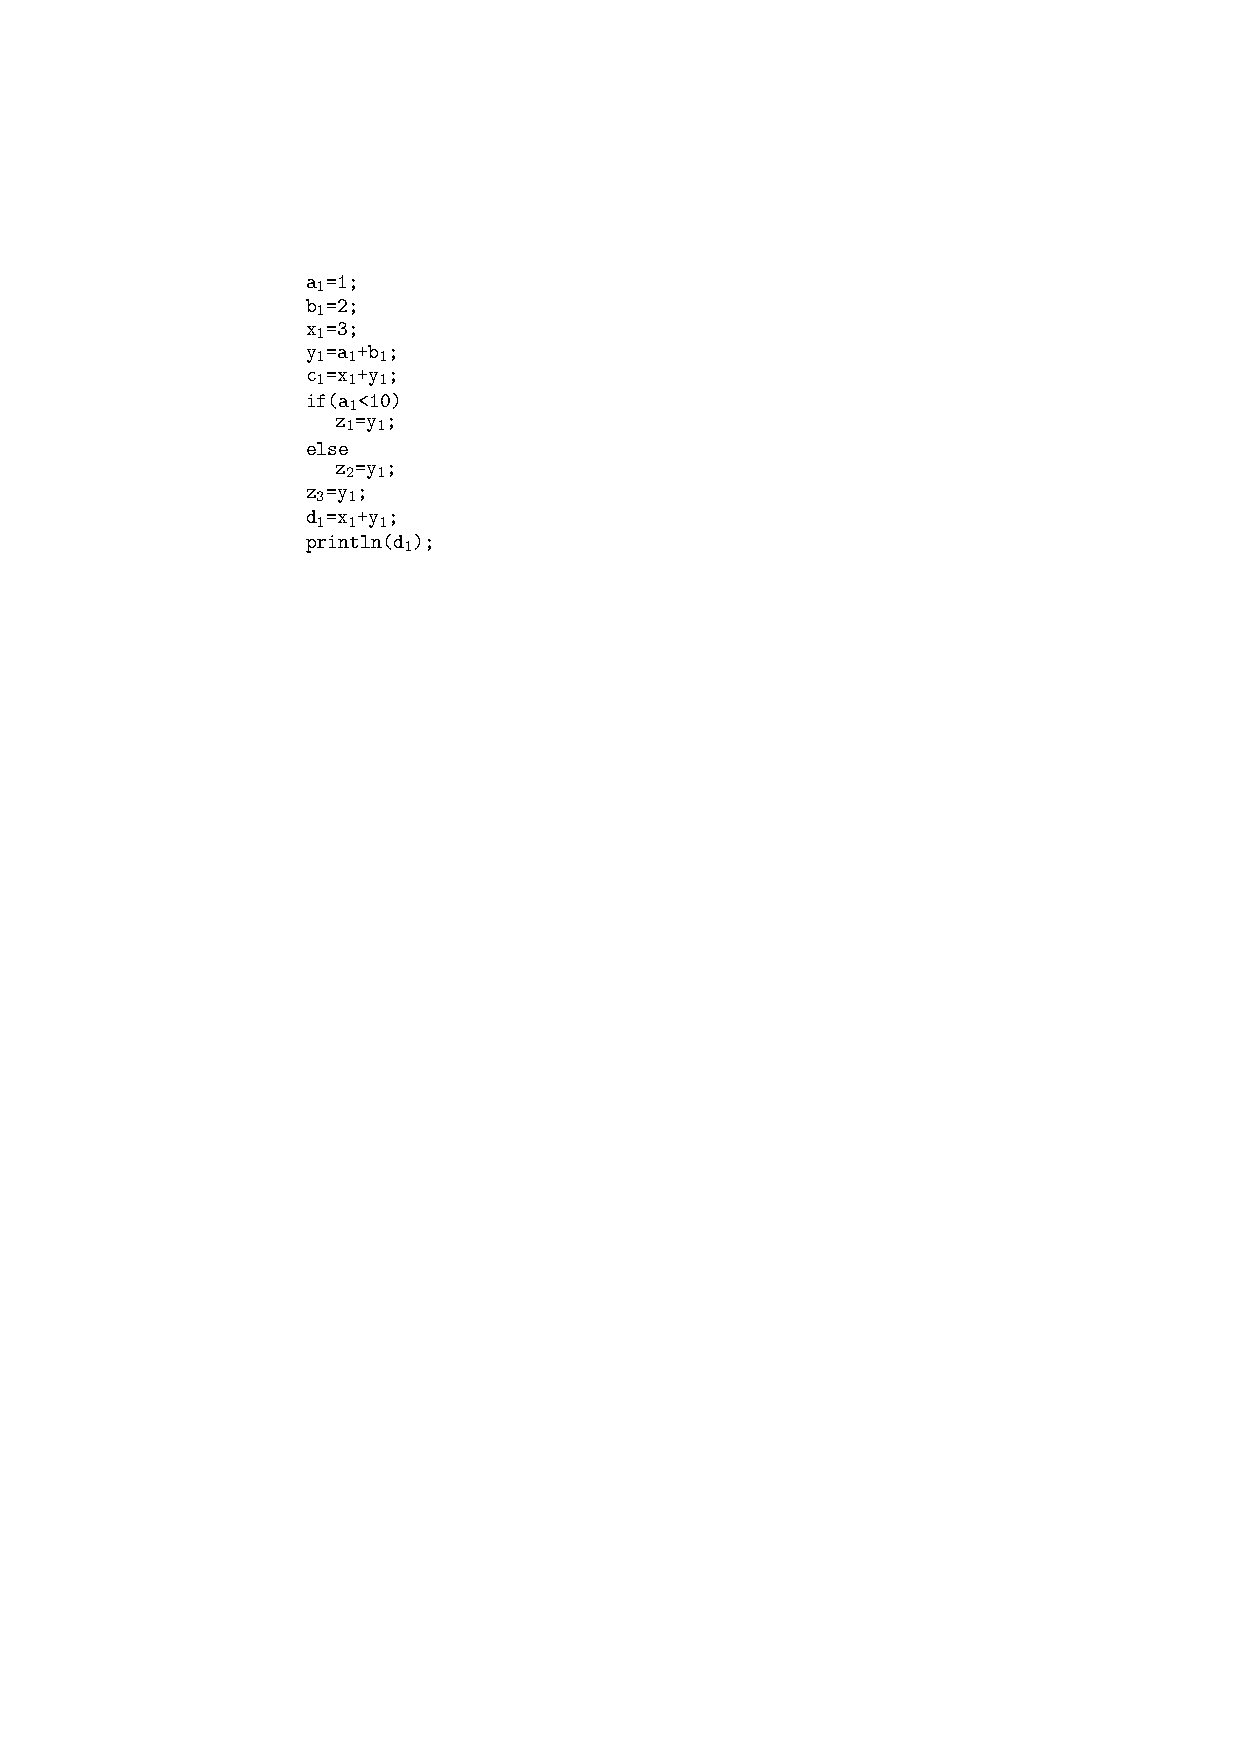
\includegraphics{ssasrc04.pdf}
           & \hspace*{1zw}$\Rightarrow$\hspace*{1zw} &
          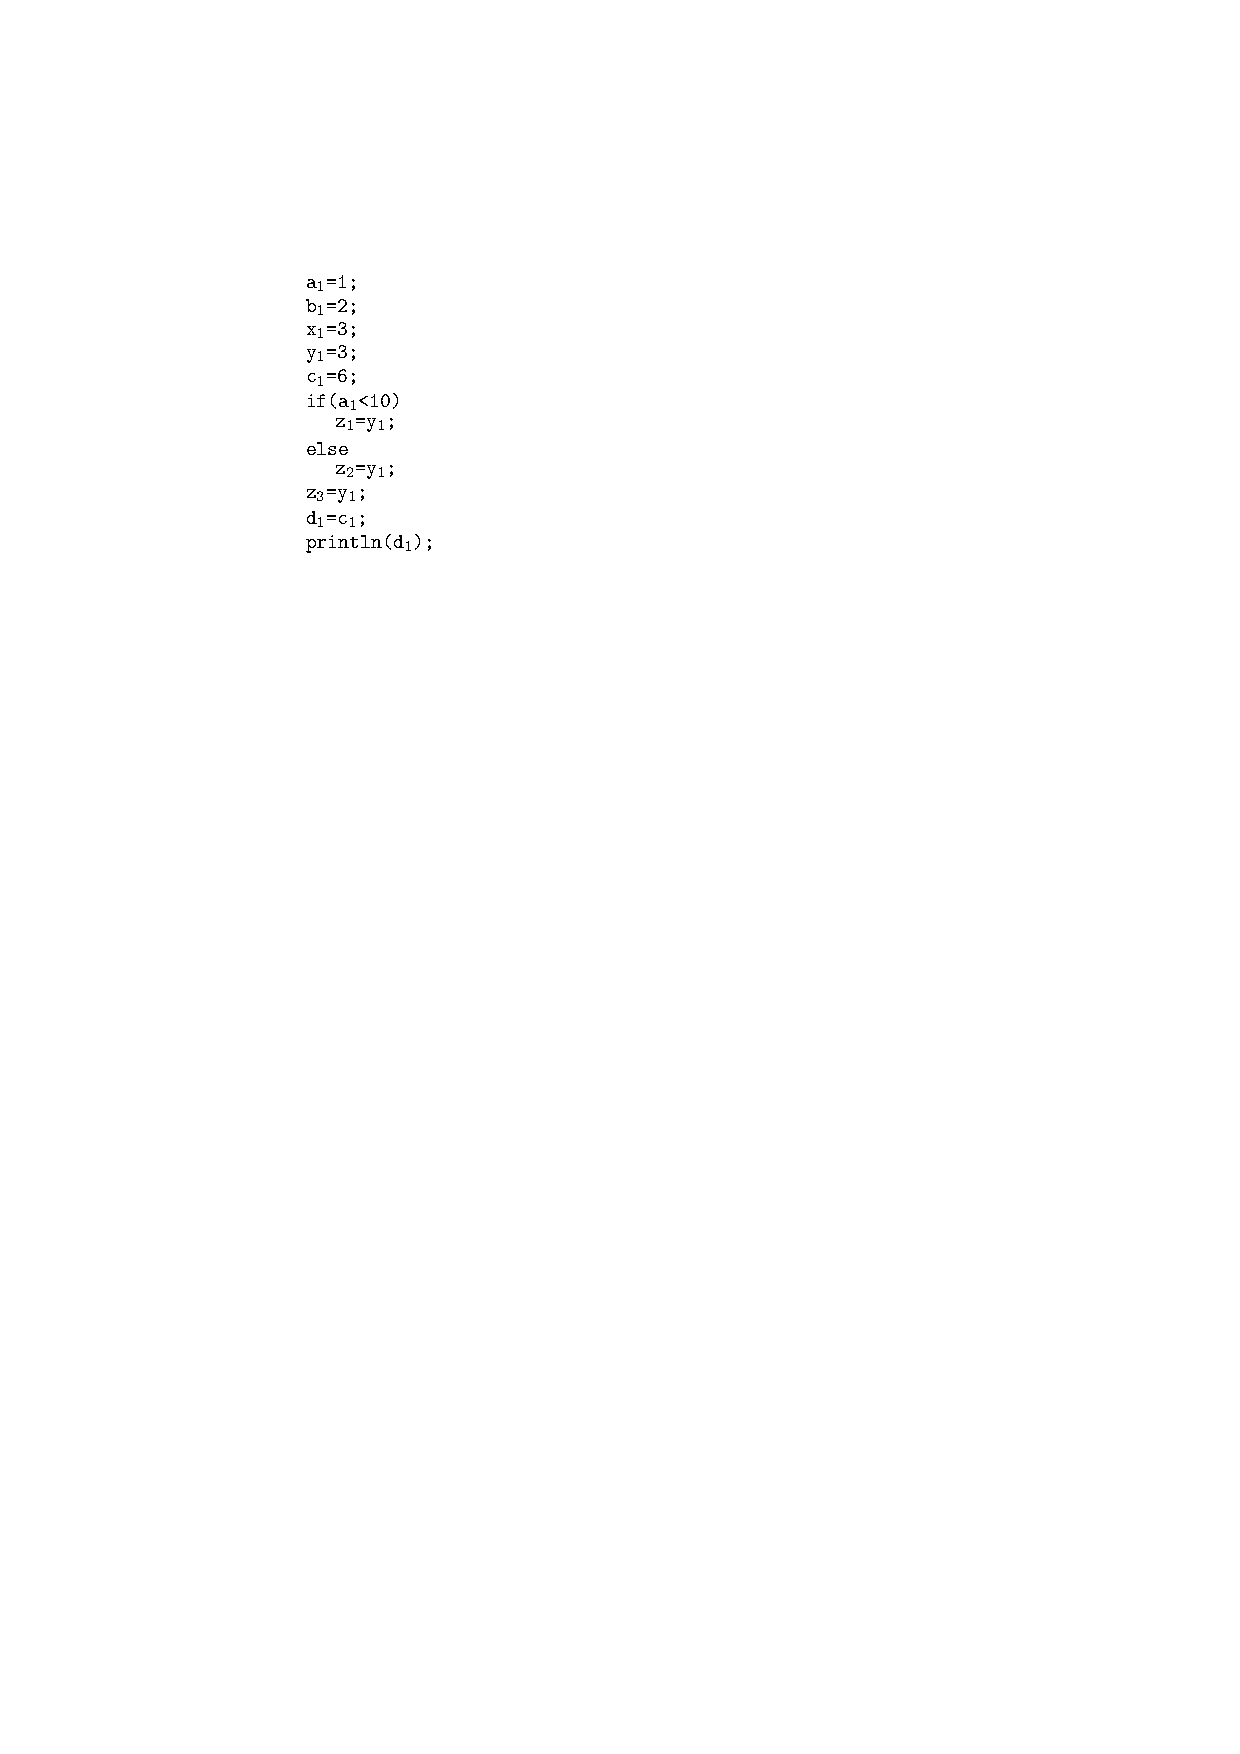
\includegraphics{ssasrc05.pdf}               \\[1zw]
          \multicolumn{3}{c}{\greentext{共通部分式除去、定数伝播}}
        \end{tabular}
      \end{center}
    \end{center}
  }

  \only<5>{
    \begin{center}
      \begin{tabular}{ccc}
        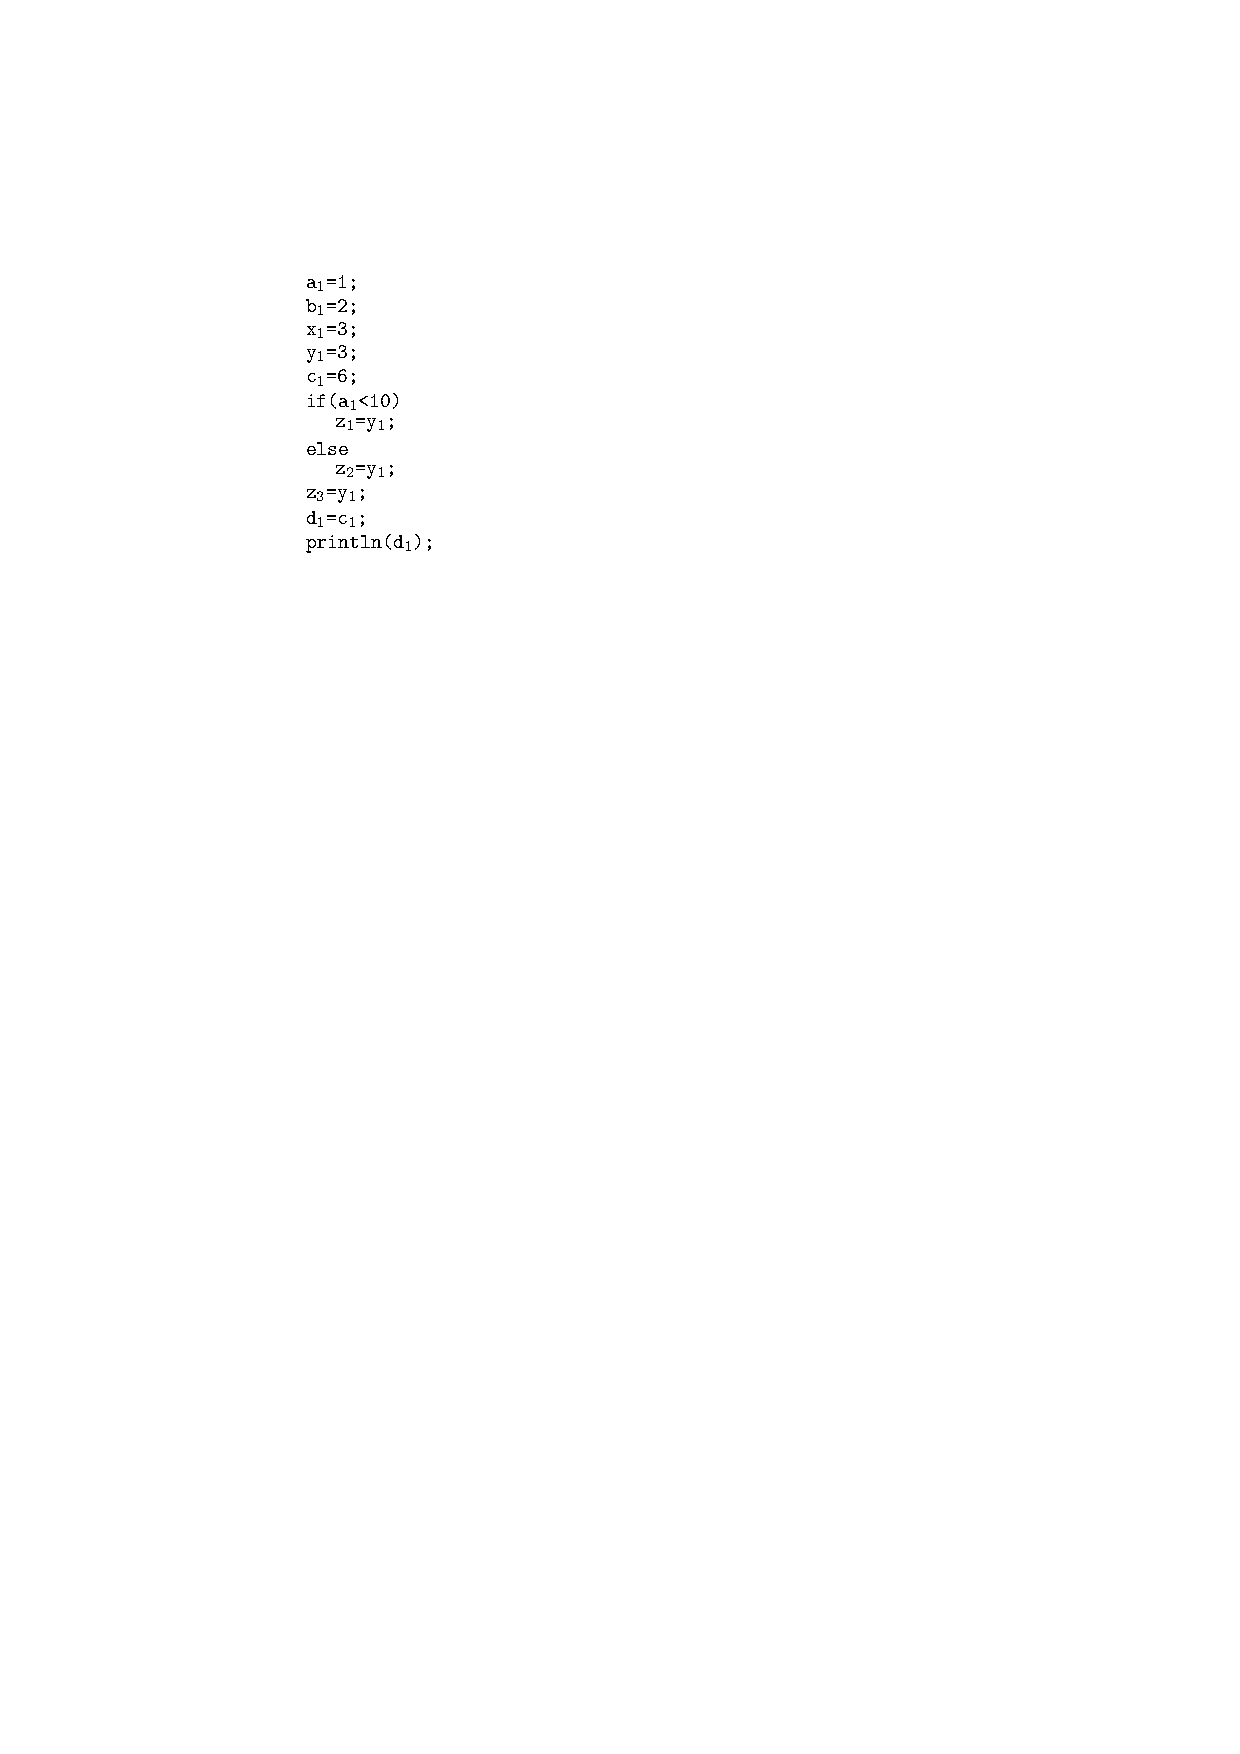
\includegraphics{ssasrc05.pdf}
         & \hspace*{1zw}$\Rightarrow$\hspace*{1zw} &
        
\includegraphics{ssasrc06.pdf}               \\[1zw]
        \multicolumn{3}{c}{\greentext{コピー伝播、定数伝播、恒等式}}
      \end{tabular}
    \end{center}
  }

\end{frame}

\begin{frame}
  \frametitle{最適化の条件}

  最適化を行うときに支配関係を壊さないようにする。

  \begin{center}
    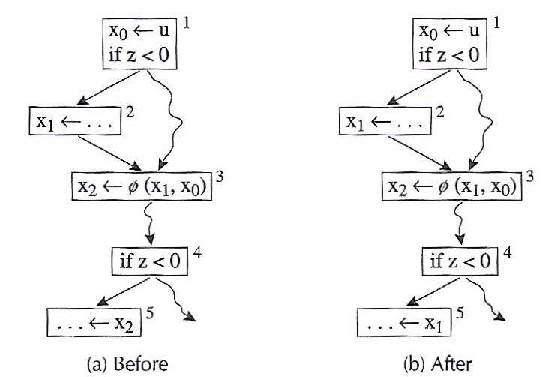
\includegraphics[height=.5\textheight]{SSAincorrectOpt.pdf}
  \end{center}

  $z<0$の評価は同じ方向にしかブランチしない\\
  $\Rightarrow$ $z<0$ならば3の$\phi$関数はいつも$x_1$を$x_2$へ代入\\
  5において$z<0$で、$x_1$を参照に用いると支配関係が壊れる\\
  (支配関係を壊すと一般にはデータフローが保証されない)\\
  \greentext{静的と動的のギャップを$\phi$関数で埋めているため}
\end{frame}

% \begin{frame}
%   \frametitle{条件付き定数伝播}
%   \begin{center}
%     {\begin{tabularx}{.75\textwidth}{XXX}
%       \multicolumn{1}{m{.35\textwidth}}{
%       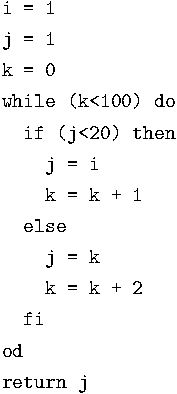
\includegraphics[height=.7\textheight]{prog-example-crop.pdf}
%       }
%       & \multicolumn{1}{m{2em}}{$\Rightarrow$} &
%       \multicolumn{1}{m{.4\textwidth}}{
%       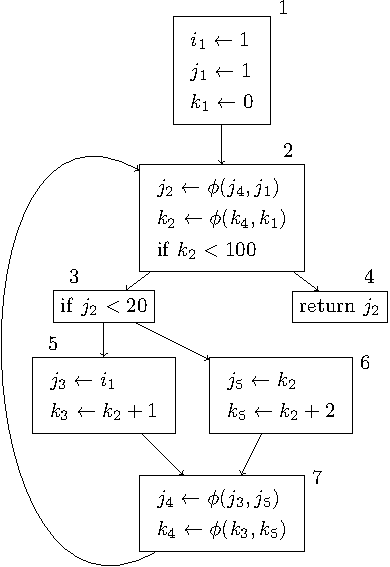
\includegraphics[height=.7\textheight]{SSA-prog-crop.pdf}
%       }
%      \end{tabularx}}
%   \end{center}
%   \centerline{\greentext{6のブロックは実行されるか？}}
% \end{frame}

% \begin{frame}
%   \frametitle{条件付き定数伝播アルゴリズム}
%   {\scriptsize
%   \begin{tabular}{l}
%   $\mathcal{B}[n]=true$ならばブロック$n$は実行される可能性あり\\
%   $\mathcal{V}[x]$ 定数$c$, 決まらない$\top$, 初期化されない$\bot$
%   \end{tabular}}

%   \vspace*{5pt}

%   {\scriptsize\color[rgb]{0,0.5,0}
%   $\phi(x_1,\ldots,x_n)$において，$x_i$のフロー元となる直近のブロックを$b_i$と書く．
%   }

%   \vspace*{5pt}

%   {\scriptsize
%   初期化：$\mathcal{B}[n]=false$ ($1\leq n\leq N$), 
%   $\mathcal{V}[x]=\bot$ ($x\in X$)
%   }

%   \vspace*{5pt}

%   {\scriptsize 
%   \begin{list}{Step \arabic{coffee}.}{\usecounter{coffee}}
%     \item 実行の引数となる変数$x\in P$について，$\mathcal{V}(x)\leftarrow\top$ 
%     \item $\mathcal{B}[1]\leftarrow true$
%   \end{list}
%   $\mathcal{B}$と$\mathcal{V}$が変化しなくなるまでStep 3 $\sim$ Step 10を繰り返す．
%   \begin{list}{Step \arabic{coffee}.}{\usecounter{coffee}\setcounter{coffee}{2}}
%     \item
%     $\mathcal{B}[n]=true$の次のブロックが唯一の$m$のとき，
%     $\mathcal{B}[m]\leftarrow true$
%     \item $z\leftarrow x\; op\; y$に対して$\mathcal{V}[x]=c_1$ かつ $\mathcal{V}[y]=c_2$
%     のとき，$\mathcal{V}[z]\leftarrow c_1\; op\; c_2$
%     \item $z\leftarrow x\; op\; y$に対して$\mathcal{V}[x]=\top$ または $\mathcal{V}[y]=\top$
%     のとき，$\mathcal{V}[z]\leftarrow\top$
%     \item $y\leftarrow\phi(x_1,\ldots,x_n)$に対して，
%     $\mathcal{V}[x_i]=c_i$, $\mathcal{V}[x_j]=c_j$, $c_i\not=c_j$となる
%     $i,j$が存在し，$\mathcal{B}[b_i]=\mathcal{B}[b_j]=true$のとき，$y\leftarrow\top$
%     \item $y\leftarrow\phi(x_1,\ldots,x_n)$に対して，
%     $\mathcal{V}[x_i]=\top$となる$i$が存在するならば$\mathcal{V}[y]=\top$
%     \item $y\leftarrow\phi(x_1,\ldots,x_n)$に対して，
%     $\mathcal{B}[b_i]=true$である$x_i$ですべて$\mathcal{V}[x_i]=c$であり，
%     $\mathcal{B}[b_j]=false$である$x_j$ですべて$\mathcal{V}[x_j]=\bot$ならば，
%     $\mathcal{V}[y]\leftarrow c$
%     \item $\mathbf{if}\ x<y\ \mathbf{goto}\ B_i\ \mathbf{else}\ B_j$に対して
%     $\mathcal{V}[x]=\top$ または $\mathcal{V}[y]=\top$ならば
%     $\mathcal{B}[i]\leftarrow true$, $\mathcal{B}[j]\leftarrow true$
%     \item $\mathbf{if}\ x<y\ \mathbf{goto}\ B_i\ \mathbf{else}\ B_j$に対して
%     $\mathcal{V}[x]=c_1$, $\mathcal{V}[y]=c_2$のとき，$c_1<c_2$ならば
%     $\mathcal{B}[i]\leftarrow true$, $c_1\not<c_2$ならば$\mathcal{B}[j]\leftarrow true$.
%   \end{list}
%   }

% \end{frame}

% \begin{frame}
% \frametitle{条件付き定数伝播}

% \begin{center}
%   \begin{tabularx}{.6\textwidth}{cc}
%     \multicolumn{1}{m{.3\textwidth}}{
%      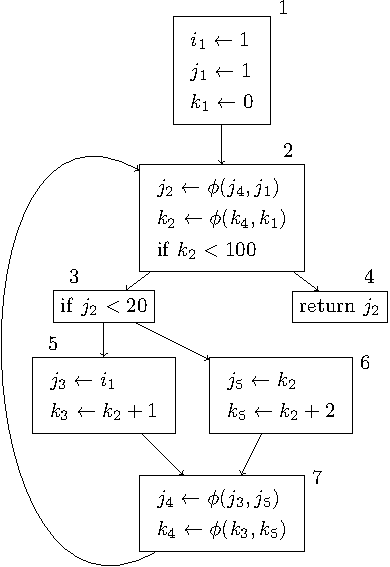
\includegraphics[width=.3\textwidth]{SSA-prog-crop.pdf}
%      }
%      &
%      {\small
%      \begin{tabularx}{0.3\textwidth}{XXXXX}
%        $B$ & $\mathcal{E}[B]$ & & $x$ & $\mathcal{V}[x]$\\\cline{1-2}\cline{4-5}
%        1 & $true$ & & $i_1$ & $1$\\
%        2 & $true$ & & $j_1$ & $1$\\
%        3 & $true$ & & $j_2$ & $1$\\
%        4 & $true$ & & $j_3$ & $1$\\
%        5 & $true$ & & $j_4$ & $1$\\
%        6 & $false$ & & $j_5$ & $\bot$\\
%        7 & $true$ & & $k_1$ & $0$\\
%          &        & & $k_2$ & $\top$\\
%          &        & & $k_3$ & $\top$\\
%          &        & & $k_4$ & $\top$\\
%          &        & & $k_5$ & $\bot$
%      \end{tabularx}}
%    \end{tabularx}
%    \end{center}
%    \greentext{$j$は定数が伝播して，$j<20$の判定がいつも成立．$k$は$\top$なので$k<100$の
%    判定は実行時}
% \end{frame}

% \begin{frame}
%   \frametitle{条件付き定数伝播}
%   \begin{center}
%     \begin{tabularx}{0.8\textwidth}{XXX}
%       \multicolumn{1}{m{.3\textwidth}}{
%         \only<1>{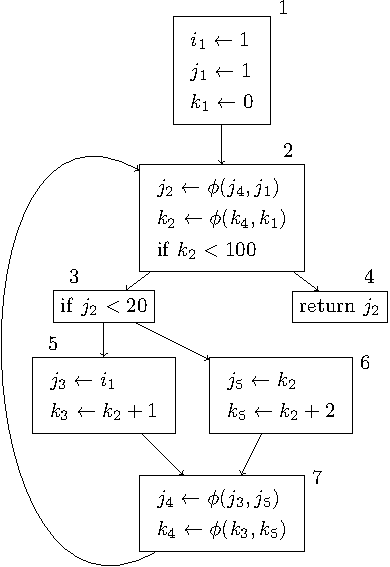
\includegraphics[width=.3\textwidth]{SSA-prog-crop.pdf}}
%         \only<2>{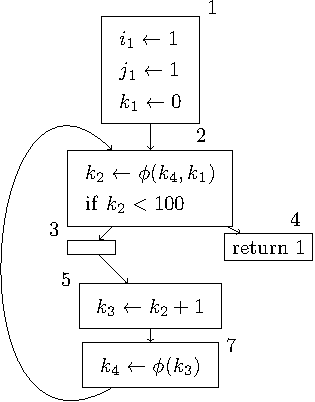
\includegraphics[width=.3\textwidth]{SSA-prog-opt1-crop.pdf}}
%       }
%       &
%       \multicolumn{1}{m{2em}}{$\Rightarrow$} 
%       &
%       \multicolumn{1}{m{.3\textwidth}}
%       {
%         \only<1>{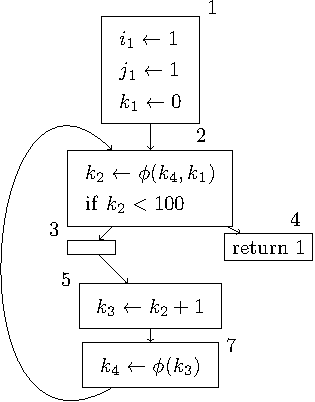
\includegraphics[width=.3\textwidth]{SSA-prog-opt1-crop.pdf}}
%         \only<2>{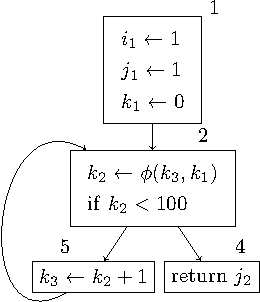
\includegraphics[width=.3\textwidth]{SSA-prog-opt2-crop.pdf}}
%       }
%     \end{tabularx}
%   \end{center}
% \end{frame}

\subsection{SSA形式からの逆変換}

\begin{frame}
  \frametitle{SSA形式からの逆変換：$\phi$関数の消去}

  \begin{tabular}{ccc}
    \begin{minipage}{.4\textwidth}
      \begin{tikzpicture}
        \node[draw] (u1) at (0,2) {$x_1=\cdots$};
        \node[draw] (u2) at (2,2) {$x_2=\cdots$};
        \node[draw] (v0) at (1,0) {$x_3=\phi(x_1,x_2)$};
        \path[->] (u1) edge (v0) (u2) edge (v0);
        \node at ($(u1)+(-1,0)$) {$u_1$};
        \node at ($(u2)+(-1,0)$) {$u_2$};
        \node at ($(v0)+(-1.5,0)$) {$v$};
      \end{tikzpicture}
    \end{minipage}
     & $\Rightarrow$ &
    \begin{minipage}{.4\textwidth}
      \begin{tikzpicture}
        \node[style=dashed,draw] (uu1) at (0,2) {$x_1=\cdots$};
        \node[style=dotted,draw] (uw1) at (0,1) {$x_3=x_1$};
        \node[style=dashed,draw] (uu2) at (2.5,2) {$x_2=\cdots$};
        \node[style=dotted,draw] (uw2) at (2.5,1) {$x_3=x_2$};
        \node at ($(uu1)+(-1.1,0)$) {$u_1$};
        \node at ($(uw1)+(-1.1,0)$) {$w_1$};
        \node at ($(uu2)+(-1.1,0)$) {$u_2$};
        \node at ($(uw2)+(-1.1,0)$) {$w_2$};
        \node[minimum width=1.5cm, minimum height=5mm,draw] (ww1) at (1.25,0) {};
        \node at ($(ww1)+(-1.1,0)$) {$v$};
        \draw (-0.9,0.6) rectangle +(1.8,1.8);
        \draw (1.6,0.6) rectangle +(1.8,1.8);
        \path[->](uu1) edge (uw1)  (uu2) edge (uw2) (uw1) edge (ww1)  (uw2) edge (ww1);
      \end{tikzpicture}
    \end{minipage}
  \end{tabular}

  \vspace*{10pt}

  \redtext{$\phi$関数に対してはコード生成ができない。}

  \vspace*{5pt}

  \greentext{(先の例はたまたま$\phi$関数まで消えてしまった。)}

  \vspace*{1zw}

  \greentext{ノード$w_1$,$w_2$を挿入して、$\phi$関数を消去}

  \vspace*{10pt}

  3番地コード$\rightarrow$SSA形式$\rightarrow$最適化$\rightarrow$ $\phi$関数消去

\end{frame}

\begin{frame}
  \frametitle{逆変換アルゴリズム}

  \begin{trivlist}
    \item [1.] フローグラフの変換\\
    $\phi$関数を持つブロックに対して挿入条件を満たさないまで、代
    入文を挿入する。

    \vspace*{1zw}

    挿入条件：$\phi$関数を持つブロックが複数の先行頂点を持ち、そ
    のうちの一つが複数の後続頂点を持つ。

    先行ブロックの最後がgoto文の場合は、goto文の直前に代入文を挿
    入する。
    \item [2.] $\phi$関数の消去
  \end{trivlist}

\end{frame}

\begin{frame}
  \frametitle{逆変換例}

  %\greentext{(p.136 演習問題3)}

  \only<1>{
    \begin{center}
      \scalebox{0.75}{
        \begin{tikzpicture}
          \node[anchor=west,draw,minimum width=3.8cm] (v0) at (0,6.5)
          {\small $\begin{array}{ll}\hspace*{1zw}
                 & \mathtt{i_1=1}                              \\[-2pt]
                 & \mathtt{j_1=1}                              \\[-2pt]
                 & \mathtt{k_1=1}                              \\[-2pt]
                 & \mathtt{if}\ p'\ \mathtt{goto}\ \mathtt{L1} \\\end{array}$};
          \node at ($(v0)+(-2.2,0.7)$) {$v_0$};
          \node[anchor=west,draw,minimum width=3.8cm] (v1) at (0,4.25)
          {\small $\begin{array}{ll}
                L3: & \mathtt{i_2=}\phi\mathtt{(i_1,i_3)}        \\[-2pt]
                    & \mathtt{if}\ q\ \mathtt{goto}\ \mathtt{L2} \\
              \end{array}$};
          \node at ($(v1)+(-2.2,0)$) {$v_1$};
          \node[anchor=west,draw,minimum width=3.8cm] (v2) at (0,2.5)
          {\small $\begin{array}{ll}
                \hspace*{1zw} & \mathtt{i_3=i_2+1} \\
                              & \mathtt{goto\ L3}
              \end{array}$};
          \node at ($(v2)+(-2.2,0.2)$) {$v_2$};
          \node[anchor=west,draw,minimum width=3.8cm] (v3) at (0,1)
          {\small $\begin{array}{ll}
                L1: & \mathtt{j_2=i_1+k_1} \\
              \end{array}$};
          \node at ($(v3)+(-2.2,0)$) {$v_3$};
          \node[anchor=west,draw,minimum width=3.8cm] (v4) at (0,-0.5)
          {\small $\begin{array}{ll}
                L2: & \mathtt{i_4=}\phi\mathtt{(i_2,i_1)} \\
                    & \mathtt{j_3=}\phi\mathtt{(j_1,j_2)} \\
                    & \mathtt{k_2=i_4+j_3}                \\
              \end{array}$};
          \node at ($(v4)+(-2.2,0)$) {$v_4$};
          \path[->] (v0) edge (v1);
          \path[->] (v1) edge (v2);
          \path[->] (v2) [out=210,in=150,looseness=3] edge (v1);
          \path[->] (v0) [out=350,in=10,looseness=0.5] edge (v3);
          \path[->] (v1) [out=350,in=10,looseness=0.5] edge (v4);
          \path[->] (v3) edge (v4);
        \end{tikzpicture}
      }
    \end{center}
  }
  \only<2>{
    \scalebox{0.8}{
      \begin{tikzpicture}
        \node[anchor=west,draw,minimum width=3.8cm] (v0) at (0,6.5)
        {\small $\begin{array}{ll}\hspace*{1zw}
               & \mathtt{i_1=1}                              \\[-2pt]
               & \mathtt{j_1=1}                              \\[-2pt]
               & \mathtt{k_1=1}                              \\[-2pt]
               & \mathtt{if}\ p'\ \mathtt{goto}\ \mathtt{L1} \\\end{array}$};
        \node at ($(v0)+(-2.2,0.7)$) {$v_0$};
        \node[anchor=west,draw, minimum width=3.8cm,minimum height=5mm,fill=lightlightgrey] (w0) at (0,5)
        {$\hspace*{1zw}\mathtt{i_2=i_1}$};
        \node at ($(w0)+(-2.2,0)$) {$w_0$};
        \node[anchor=west,draw,minimum width=3.8cm] (v1) at (0,3.8)
        {$\mathtt{L3:\ if}\ q'\ \mathtt{goto}\ \mathtt{L2}$};
        \node at ($(v1)+(-2.2,0)$) {$v_1$};
        \node[anchor=west,draw,minimum width=3.8cm] (v2) at (0,2)
        {$\begin{array}{ll}\hspace*{1zw} & \mathtt{i_3=i_2+1} \\[-2pt]
                               & \mathtt{i_2=i_3}   \\[-2pt]
                               & goto\ L3\end{array}$};
        \node at ($(v2)+(-2.2,0.6)$) {$v_2$};
        \node[anchor=west,draw,minimum width=3cm,minimum height=8mm,fill=lightlightgrey] (w1) at (5,2)
        {$\begin{array}{ll}L2: & \mathtt{i_4=i_2} \\[-2pt] & \mathtt{j_3=j_1}\\[-2pt]
                     & goto\ L4
            \end{array}$};
        \node at ($(w1)+(-1.8,0.3)$) {$w_1$};
        \node[anchor=west,draw,minimum width=3.8cm] (v3) at (9,4)
        {$\begin{array}{ll}L1: & \mathtt{j_2=i_1+k_1} \\
                     & \mathtt{i_4=j_1}     \\ & \mathtt{j_3=j_2}\end{array}$};
        \node at ($(v3)+(-2.2,0.4)$) {$v_3$};
        \node[anchor=west,draw,minimum width=3.8cm] (v4) at (9,0)
        {$L4:$\ $\mathtt{k_2=i_4+j_3}$};
        \node at ($(v4)+(-2.2,0)$) {$v_4$};
        \path[->] (v0) edge (w0)  (w0) edge (v1)  (v1) edge (v2)  (v2) [out=190,in=170,looseness=1] edge (v1);
        \path[->] (v1) [out=350,in=135] edge (w1)  (w1) [out=330,in=120] edge (v4);
        \path[->] (v3) edge (v4);
        \path[->] (v0) [out=330,in=135] edge (v3);
      \end{tikzpicture}
    }
  }
\end{frame}

\end{document}
